\documentclass[twoside]{book}

% Packages required by doxygen
\usepackage{fixltx2e}
\usepackage{calc}
\usepackage{doxygen}
\usepackage[export]{adjustbox} % also loads graphicx
\usepackage{graphicx}
\usepackage[utf8]{inputenc}
\usepackage{makeidx}
\usepackage{multicol}
\usepackage{multirow}
\PassOptionsToPackage{warn}{textcomp}
\usepackage{textcomp}
\usepackage[nointegrals]{wasysym}
\usepackage[table]{xcolor}

% Font selection
\usepackage[T1]{fontenc}
\usepackage[scaled=.90]{helvet}
\usepackage{courier}
\usepackage{amssymb}
\usepackage{sectsty}
\renewcommand{\familydefault}{\sfdefault}
\allsectionsfont{%
  \fontseries{bc}\selectfont%
  \color{darkgray}%
}
\renewcommand{\DoxyLabelFont}{%
  \fontseries{bc}\selectfont%
  \color{darkgray}%
}
\newcommand{\+}{\discretionary{\mbox{\scriptsize$\hookleftarrow$}}{}{}}

% Page & text layout
\usepackage{geometry}
\geometry{%
  a4paper,%
  top=2.5cm,%
  bottom=2.5cm,%
  left=2.5cm,%
  right=2.5cm%
}
\tolerance=750
\hfuzz=15pt
\hbadness=750
\setlength{\emergencystretch}{15pt}
\setlength{\parindent}{0cm}
\setlength{\parskip}{3ex plus 2ex minus 2ex}
\makeatletter
\renewcommand{\paragraph}{%
  \@startsection{paragraph}{4}{0ex}{-1.0ex}{1.0ex}{%
    \normalfont\normalsize\bfseries\SS@parafont%
  }%
}
\renewcommand{\subparagraph}{%
  \@startsection{subparagraph}{5}{0ex}{-1.0ex}{1.0ex}{%
    \normalfont\normalsize\bfseries\SS@subparafont%
  }%
}
\makeatother

% Headers & footers
\usepackage{fancyhdr}
\pagestyle{fancyplain}
\fancyhead[LE]{\fancyplain{}{\bfseries\thepage}}
\fancyhead[CE]{\fancyplain{}{}}
\fancyhead[RE]{\fancyplain{}{\bfseries\leftmark}}
\fancyhead[LO]{\fancyplain{}{\bfseries\rightmark}}
\fancyhead[CO]{\fancyplain{}{}}
\fancyhead[RO]{\fancyplain{}{\bfseries\thepage}}
\fancyfoot[LE]{\fancyplain{}{}}
\fancyfoot[CE]{\fancyplain{}{}}
\fancyfoot[RE]{\fancyplain{}{\bfseries\scriptsize Generated by Doxygen }}
\fancyfoot[LO]{\fancyplain{}{\bfseries\scriptsize Generated by Doxygen }}
\fancyfoot[CO]{\fancyplain{}{}}
\fancyfoot[RO]{\fancyplain{}{}}
\renewcommand{\footrulewidth}{0.4pt}
\renewcommand{\chaptermark}[1]{%
  \markboth{#1}{}%
}
\renewcommand{\sectionmark}[1]{%
  \markright{\thesection\ #1}%
}

% Indices & bibliography
\usepackage{natbib}
\usepackage[titles]{tocloft}
\setcounter{tocdepth}{3}
\setcounter{secnumdepth}{5}
\makeindex

% Hyperlinks (required, but should be loaded last)
\usepackage{ifpdf}
\ifpdf
  \usepackage[pdftex,pagebackref=true]{hyperref}
\else
  \usepackage[ps2pdf,pagebackref=true]{hyperref}
\fi
\hypersetup{%
  colorlinks=true,%
  linkcolor=blue,%
  citecolor=blue,%
  unicode%
}

% Custom commands
\newcommand{\clearemptydoublepage}{%
  \newpage{\pagestyle{empty}\cleardoublepage}%
}

\usepackage{caption}
\captionsetup{labelsep=space,justification=centering,font={bf},singlelinecheck=off,skip=4pt,position=top}

%===== C O N T E N T S =====

\begin{document}

% Titlepage & ToC
\hypersetup{pageanchor=false,
             bookmarksnumbered=true,
             pdfencoding=unicode
            }
\pagenumbering{alph}
\begin{titlepage}
\vspace*{7cm}
\begin{center}%
{\Large Call\+Recorder }\\
\vspace*{1cm}
{\large Generated by Doxygen 1.8.13}\\
\end{center}
\end{titlepage}
\clearemptydoublepage
\pagenumbering{roman}
\tableofcontents
\clearemptydoublepage
\pagenumbering{arabic}
\hypersetup{pageanchor=true}

%--- Begin generated contents ---
\chapter{Hierarchical Index}
\section{Class Hierarchy}
This inheritance list is sorted roughly, but not completely, alphabetically\+:\begin{DoxyCompactList}
\item \contentsline{section}{com.\+aykuttasil.\+callrecord.\+Call\+Record}{\pageref{classcom_1_1aykuttasil_1_1callrecord_1_1_call_record}}{}
\item \contentsline{section}{com.\+aykuttasil.\+callrecord.\+helper.\+Prefs\+Helper}{\pageref{classcom_1_1aykuttasil_1_1callrecord_1_1helper_1_1_prefs_helper}}{}
\item Broadcast\+Receiver\begin{DoxyCompactList}
\item \contentsline{section}{com.\+aykuttasil.\+callrecord.\+receiver.\+Phone\+Call\+Receiver}{\pageref{classcom_1_1aykuttasil_1_1callrecord_1_1receiver_1_1_phone_call_receiver}}{}
\begin{DoxyCompactList}
\item \contentsline{section}{com.\+aykuttasil.\+callrecord.\+receiver.\+Call\+Record\+Receiver}{\pageref{classcom_1_1aykuttasil_1_1callrecord_1_1receiver_1_1_call_record_receiver}}{}
\end{DoxyCompactList}
\end{DoxyCompactList}
\item Service\begin{DoxyCompactList}
\item \contentsline{section}{com.\+aykuttasil.\+callrecord.\+service.\+Call\+Record\+Service}{\pageref{classcom_1_1aykuttasil_1_1callrecord_1_1service_1_1_call_record_service}}{}
\end{DoxyCompactList}
\end{DoxyCompactList}

\chapter{Class Index}
\section{Class List}
Here are the classes, structs, unions and interfaces with brief descriptions\+:\begin{DoxyCompactList}
\item\contentsline{section}{\hyperlink{classcom_1_1aykuttasil_1_1callrecord_1_1_call_record}{com.\+aykuttasil.\+callrecord.\+Call\+Record} \\*Регистрация звонков }{\pageref{classcom_1_1aykuttasil_1_1callrecord_1_1_call_record}}{}
\item\contentsline{section}{\hyperlink{classcom_1_1aykuttasil_1_1callrecord_1_1receiver_1_1_call_record_receiver}{com.\+aykuttasil.\+callrecord.\+receiver.\+Call\+Record\+Receiver} \\*Регистрация звонков }{\pageref{classcom_1_1aykuttasil_1_1callrecord_1_1receiver_1_1_call_record_receiver}}{}
\item\contentsline{section}{\hyperlink{classcom_1_1aykuttasil_1_1callrecord_1_1service_1_1_call_record_service}{com.\+aykuttasil.\+callrecord.\+service.\+Call\+Record\+Service} \\*Регистрация звонков }{\pageref{classcom_1_1aykuttasil_1_1callrecord_1_1service_1_1_call_record_service}}{}
\item\contentsline{section}{\hyperlink{classcom_1_1aykuttasil_1_1callrecord_1_1receiver_1_1_phone_call_receiver}{com.\+aykuttasil.\+callrecord.\+receiver.\+Phone\+Call\+Receiver} \\*Регистрация звонков }{\pageref{classcom_1_1aykuttasil_1_1callrecord_1_1receiver_1_1_phone_call_receiver}}{}
\item\contentsline{section}{\hyperlink{classcom_1_1aykuttasil_1_1callrecord_1_1helper_1_1_prefs_helper}{com.\+aykuttasil.\+callrecord.\+helper.\+Prefs\+Helper} \\*Регистрация звонков }{\pageref{classcom_1_1aykuttasil_1_1callrecord_1_1helper_1_1_prefs_helper}}{}
\end{DoxyCompactList}

\chapter{Class Documentation}
\hypertarget{classcom_1_1aykuttasil_1_1callrecord_1_1_call_record}{}\section{com.\+aykuttasil.\+callrecord.\+Call\+Record Class Reference}
\label{classcom_1_1aykuttasil_1_1callrecord_1_1_call_record}\index{com.\+aykuttasil.\+callrecord.\+Call\+Record@{com.\+aykuttasil.\+callrecord.\+Call\+Record}}


Регистрация звонков.  


\subsection*{Classes}
\begin{DoxyCompactItemize}
\item 
class {\bfseries Builder}
\end{DoxyCompactItemize}
\subsection*{Public Member Functions}
\begin{DoxyCompactItemize}
\item 
void \hyperlink{classcom_1_1aykuttasil_1_1callrecord_1_1_call_record_ab7603981df60fd6c66fdc8692ca08ee6}{start\+Call\+Receiver} ()
\item 
void \hyperlink{classcom_1_1aykuttasil_1_1callrecord_1_1_call_record_a269eed369eac397c04aca3176c0715f7}{stop\+Call\+Receiver} ()
\item 
void \hyperlink{classcom_1_1aykuttasil_1_1callrecord_1_1_call_record_a1d82c1d77cf1bec400c1e281b8730075}{start\+Call\+Record\+Service} ()
\item 
void \hyperlink{classcom_1_1aykuttasil_1_1callrecord_1_1_call_record_a8ffc1079f79fcfc9ef2ef2c17f030173}{enable\+Save\+File} ()
\item 
void \hyperlink{classcom_1_1aykuttasil_1_1callrecord_1_1_call_record_ae1bb1b4b4b0dd8012a4443d8c7ea5319}{disable\+Save\+File} ()
\item 
boolean \hyperlink{classcom_1_1aykuttasil_1_1callrecord_1_1_call_record_a3fe28aee7367f67e6d34a11dcdd10673}{get\+State\+Save\+File} ()
\item 
void \hyperlink{classcom_1_1aykuttasil_1_1callrecord_1_1_call_record_a46f071e0d6c3d9f2fd87cce016b74aad}{change\+Record\+File\+Name} (String new\+File\+Name)
\item 
String \hyperlink{classcom_1_1aykuttasil_1_1callrecord_1_1_call_record_a05ca6a80ce9f6477b5ab6c8475eb6867}{get\+Record\+File\+Name} ()
\item 
void \hyperlink{classcom_1_1aykuttasil_1_1callrecord_1_1_call_record_a4d821dd8af3aecba6f2618f799099cb9}{change\+Record\+Dir\+Name} (String new\+Dir\+Name)
\item 
String \hyperlink{classcom_1_1aykuttasil_1_1callrecord_1_1_call_record_a9a68d111ed8cf646ac90fe8cb32ffacb}{get\+Record\+Dir\+Name} ()
\item 
void \hyperlink{classcom_1_1aykuttasil_1_1callrecord_1_1_call_record_a431bf7816cd1f9a635f2eaf7dc9514f2}{change\+Record\+Dir\+Path} (String new\+Dir\+Path)
\item 
String \hyperlink{classcom_1_1aykuttasil_1_1callrecord_1_1_call_record_a71b3661c65db0f8c87522aa85a1d6f7c}{get\+Record\+Dir\+Path} ()
\item 
void \hyperlink{classcom_1_1aykuttasil_1_1callrecord_1_1_call_record_a0b6b62b01721308ebcdbaf3c078aa2fa}{change\+Receiver} (\hyperlink{classcom_1_1aykuttasil_1_1callrecord_1_1receiver_1_1_call_record_receiver}{Call\+Record\+Receiver} receiver)
\end{DoxyCompactItemize}
\subsection*{Static Public Member Functions}
\begin{DoxyCompactItemize}
\item 
static \hyperlink{classcom_1_1aykuttasil_1_1callrecord_1_1_call_record}{Call\+Record} \hyperlink{classcom_1_1aykuttasil_1_1callrecord_1_1_call_record_acf60d04b55e69ddc6489a2c0e06a2f36}{init\+Receiver} (Context context)
\item 
static \hyperlink{classcom_1_1aykuttasil_1_1callrecord_1_1_call_record}{Call\+Record} \hyperlink{classcom_1_1aykuttasil_1_1callrecord_1_1_call_record_a58717cda16f688a875a0e32f03d3dbbc}{init\+Service} (Context context)
\end{DoxyCompactItemize}
\subsection*{Static Public Attributes}
\begin{DoxyCompactItemize}
\item 
\mbox{\Hypertarget{classcom_1_1aykuttasil_1_1callrecord_1_1_call_record_a4199078f7f57ac7c0580f27cda014e41}\label{classcom_1_1aykuttasil_1_1callrecord_1_1_call_record_a4199078f7f57ac7c0580f27cda014e41}} 
static final String \hyperlink{classcom_1_1aykuttasil_1_1callrecord_1_1_call_record_a4199078f7f57ac7c0580f27cda014e41}{P\+R\+E\+F\+\_\+\+S\+A\+V\+E\+\_\+\+F\+I\+LE} = \char`\"{}Pref\+Save\+File\char`\"{}
\begin{DoxyCompactList}\small\item\em константа для сохранения файла \end{DoxyCompactList}\item 
\mbox{\Hypertarget{classcom_1_1aykuttasil_1_1callrecord_1_1_call_record_ab4600912a0eaf76f06353f3b40a81746}\label{classcom_1_1aykuttasil_1_1callrecord_1_1_call_record_ab4600912a0eaf76f06353f3b40a81746}} 
static final String \hyperlink{classcom_1_1aykuttasil_1_1callrecord_1_1_call_record_ab4600912a0eaf76f06353f3b40a81746}{P\+R\+E\+F\+\_\+\+F\+I\+L\+E\+\_\+\+N\+A\+ME} = \char`\"{}Pref\+File\+Name\char`\"{}
\begin{DoxyCompactList}\small\item\em константа для сохранения имени файла \end{DoxyCompactList}\item 
\mbox{\Hypertarget{classcom_1_1aykuttasil_1_1callrecord_1_1_call_record_a625b7daac21b3dc9dda745cf21a447cb}\label{classcom_1_1aykuttasil_1_1callrecord_1_1_call_record_a625b7daac21b3dc9dda745cf21a447cb}} 
static final String \hyperlink{classcom_1_1aykuttasil_1_1callrecord_1_1_call_record_a625b7daac21b3dc9dda745cf21a447cb}{P\+R\+E\+F\+\_\+\+D\+I\+R\+\_\+\+N\+A\+ME} = \char`\"{}Pref\+Dir\+Name\char`\"{}
\begin{DoxyCompactList}\small\item\em константа для сохранения имени директории \end{DoxyCompactList}\item 
\mbox{\Hypertarget{classcom_1_1aykuttasil_1_1callrecord_1_1_call_record_a68e254b4a0603e6531c297bde62faddb}\label{classcom_1_1aykuttasil_1_1callrecord_1_1_call_record_a68e254b4a0603e6531c297bde62faddb}} 
static final String \hyperlink{classcom_1_1aykuttasil_1_1callrecord_1_1_call_record_a68e254b4a0603e6531c297bde62faddb}{P\+R\+E\+F\+\_\+\+D\+I\+R\+\_\+\+P\+A\+TH} = \char`\"{}Pref\+Dir\+Path\char`\"{}
\begin{DoxyCompactList}\small\item\em константа для сохранения пути до директории \end{DoxyCompactList}\item 
\mbox{\Hypertarget{classcom_1_1aykuttasil_1_1callrecord_1_1_call_record_ac9a6ae5d187f63d213a6d8f9ffb31d37}\label{classcom_1_1aykuttasil_1_1callrecord_1_1_call_record_ac9a6ae5d187f63d213a6d8f9ffb31d37}} 
static final String \hyperlink{classcom_1_1aykuttasil_1_1callrecord_1_1_call_record_ac9a6ae5d187f63d213a6d8f9ffb31d37}{P\+R\+E\+F\+\_\+\+S\+H\+O\+W\+\_\+\+S\+E\+ED} = \char`\"{}Pref\+Show\+Seed\char`\"{}
\begin{DoxyCompactList}\small\item\em константа, непанятна зачем нужна \end{DoxyCompactList}\item 
\mbox{\Hypertarget{classcom_1_1aykuttasil_1_1callrecord_1_1_call_record_ab0484fa6142468ce2c17ebc3b8c276c7}\label{classcom_1_1aykuttasil_1_1callrecord_1_1_call_record_ab0484fa6142468ce2c17ebc3b8c276c7}} 
static final String \hyperlink{classcom_1_1aykuttasil_1_1callrecord_1_1_call_record_ab0484fa6142468ce2c17ebc3b8c276c7}{P\+R\+E\+F\+\_\+\+S\+H\+O\+W\+\_\+\+P\+H\+O\+N\+E\+\_\+\+N\+U\+M\+B\+ER} = \char`\"{}Pref\+Show\+Phone\+Number\char`\"{}
\begin{DoxyCompactList}\small\item\em константа для отображения номера телефона \end{DoxyCompactList}\item 
\mbox{\Hypertarget{classcom_1_1aykuttasil_1_1callrecord_1_1_call_record_ab42416e630439cf8681ad22afdb55255}\label{classcom_1_1aykuttasil_1_1callrecord_1_1_call_record_ab42416e630439cf8681ad22afdb55255}} 
static final String \hyperlink{classcom_1_1aykuttasil_1_1callrecord_1_1_call_record_ab42416e630439cf8681ad22afdb55255}{P\+R\+E\+F\+\_\+\+A\+U\+D\+I\+O\+\_\+\+S\+O\+U\+R\+CE} = \char`\"{}Pref\+Audio\+Source\char`\"{}
\begin{DoxyCompactList}\small\item\em константа для задания источника записи \end{DoxyCompactList}\item 
\mbox{\Hypertarget{classcom_1_1aykuttasil_1_1callrecord_1_1_call_record_a348fa9cd2f19a89da0aa23c7414dd70d}\label{classcom_1_1aykuttasil_1_1callrecord_1_1_call_record_a348fa9cd2f19a89da0aa23c7414dd70d}} 
static final String \hyperlink{classcom_1_1aykuttasil_1_1callrecord_1_1_call_record_a348fa9cd2f19a89da0aa23c7414dd70d}{P\+R\+E\+F\+\_\+\+A\+U\+D\+I\+O\+\_\+\+E\+N\+C\+O\+D\+ER} = \char`\"{}Pref\+Audio\+Encoder\char`\"{}
\begin{DoxyCompactList}\small\item\em константа для задания аудио кодека \end{DoxyCompactList}\item 
\mbox{\Hypertarget{classcom_1_1aykuttasil_1_1callrecord_1_1_call_record_a76cd4ba494164060413e68f69c137d79}\label{classcom_1_1aykuttasil_1_1callrecord_1_1_call_record_a76cd4ba494164060413e68f69c137d79}} 
static final String \hyperlink{classcom_1_1aykuttasil_1_1callrecord_1_1_call_record_a76cd4ba494164060413e68f69c137d79}{P\+R\+E\+F\+\_\+\+O\+U\+T\+P\+U\+T\+\_\+\+F\+O\+R\+M\+AT} = \char`\"{}Pref\+Output\+Format\char`\"{}
\begin{DoxyCompactList}\small\item\em константа для задания разрешения выходного файла \end{DoxyCompactList}\end{DoxyCompactItemize}


\subsection{Detailed Description}
Регистрация звонков. 

\begin{DoxyAuthor}{Author}
Wonder\+Worcer 
\end{DoxyAuthor}
\begin{DoxyVersion}{Version}
0.\+5 
\end{DoxyVersion}
\begin{DoxyDate}{Date}
7 марта 2017 года
\end{DoxyDate}
Класс, реализующий регистрацию звонков 

\subsection{Member Function Documentation}
\mbox{\Hypertarget{classcom_1_1aykuttasil_1_1callrecord_1_1_call_record_a0b6b62b01721308ebcdbaf3c078aa2fa}\label{classcom_1_1aykuttasil_1_1callrecord_1_1_call_record_a0b6b62b01721308ebcdbaf3c078aa2fa}} 
\index{com\+::aykuttasil\+::callrecord\+::\+Call\+Record@{com\+::aykuttasil\+::callrecord\+::\+Call\+Record}!change\+Receiver@{change\+Receiver}}
\index{change\+Receiver@{change\+Receiver}!com\+::aykuttasil\+::callrecord\+::\+Call\+Record@{com\+::aykuttasil\+::callrecord\+::\+Call\+Record}}
\subsubsection{\texorpdfstring{change\+Receiver()}{changeReceiver()}}
{\footnotesize\ttfamily void com.\+aykuttasil.\+callrecord.\+Call\+Record.\+change\+Receiver (\begin{DoxyParamCaption}\item[{\hyperlink{classcom_1_1aykuttasil_1_1callrecord_1_1receiver_1_1_call_record_receiver}{Call\+Record\+Receiver}}]{receiver }\end{DoxyParamCaption})}

Необходим для смены способа записи файлов 
\begin{DoxyParams}{Parameters}
{\em receiver} & объект, наследник Broadcast\+Receiver, необходим для реализации всевозможных событий, возникающих во время разговора \\
\hline
\end{DoxyParams}
\mbox{\Hypertarget{classcom_1_1aykuttasil_1_1callrecord_1_1_call_record_a4d821dd8af3aecba6f2618f799099cb9}\label{classcom_1_1aykuttasil_1_1callrecord_1_1_call_record_a4d821dd8af3aecba6f2618f799099cb9}} 
\index{com\+::aykuttasil\+::callrecord\+::\+Call\+Record@{com\+::aykuttasil\+::callrecord\+::\+Call\+Record}!change\+Record\+Dir\+Name@{change\+Record\+Dir\+Name}}
\index{change\+Record\+Dir\+Name@{change\+Record\+Dir\+Name}!com\+::aykuttasil\+::callrecord\+::\+Call\+Record@{com\+::aykuttasil\+::callrecord\+::\+Call\+Record}}
\subsubsection{\texorpdfstring{change\+Record\+Dir\+Name()}{changeRecordDirName()}}
{\footnotesize\ttfamily void com.\+aykuttasil.\+callrecord.\+Call\+Record.\+change\+Record\+Dir\+Name (\begin{DoxyParamCaption}\item[{String}]{new\+Dir\+Name }\end{DoxyParamCaption})}

Необходим для смены директории сохранения файлов 
\begin{DoxyParams}{Parameters}
{\em new\+Dir\+Name} & -\/ новое имя директории \\
\hline
\end{DoxyParams}
\mbox{\Hypertarget{classcom_1_1aykuttasil_1_1callrecord_1_1_call_record_a431bf7816cd1f9a635f2eaf7dc9514f2}\label{classcom_1_1aykuttasil_1_1callrecord_1_1_call_record_a431bf7816cd1f9a635f2eaf7dc9514f2}} 
\index{com\+::aykuttasil\+::callrecord\+::\+Call\+Record@{com\+::aykuttasil\+::callrecord\+::\+Call\+Record}!change\+Record\+Dir\+Path@{change\+Record\+Dir\+Path}}
\index{change\+Record\+Dir\+Path@{change\+Record\+Dir\+Path}!com\+::aykuttasil\+::callrecord\+::\+Call\+Record@{com\+::aykuttasil\+::callrecord\+::\+Call\+Record}}
\subsubsection{\texorpdfstring{change\+Record\+Dir\+Path()}{changeRecordDirPath()}}
{\footnotesize\ttfamily void com.\+aykuttasil.\+callrecord.\+Call\+Record.\+change\+Record\+Dir\+Path (\begin{DoxyParamCaption}\item[{String}]{new\+Dir\+Path }\end{DoxyParamCaption})}

Необходим для изменения директории хранения новых файлов 
\begin{DoxyParams}{Parameters}
{\em new\+Dir\+Path} & новый путь \\
\hline
\end{DoxyParams}
\mbox{\Hypertarget{classcom_1_1aykuttasil_1_1callrecord_1_1_call_record_a46f071e0d6c3d9f2fd87cce016b74aad}\label{classcom_1_1aykuttasil_1_1callrecord_1_1_call_record_a46f071e0d6c3d9f2fd87cce016b74aad}} 
\index{com\+::aykuttasil\+::callrecord\+::\+Call\+Record@{com\+::aykuttasil\+::callrecord\+::\+Call\+Record}!change\+Record\+File\+Name@{change\+Record\+File\+Name}}
\index{change\+Record\+File\+Name@{change\+Record\+File\+Name}!com\+::aykuttasil\+::callrecord\+::\+Call\+Record@{com\+::aykuttasil\+::callrecord\+::\+Call\+Record}}
\subsubsection{\texorpdfstring{change\+Record\+File\+Name()}{changeRecordFileName()}}
{\footnotesize\ttfamily void com.\+aykuttasil.\+callrecord.\+Call\+Record.\+change\+Record\+File\+Name (\begin{DoxyParamCaption}\item[{String}]{new\+File\+Name }\end{DoxyParamCaption})}

Необходим для смены имени записываемого файла 
\begin{DoxyParams}{Parameters}
{\em new\+File\+Name} & новое имя файла \\
\hline
\end{DoxyParams}
\mbox{\Hypertarget{classcom_1_1aykuttasil_1_1callrecord_1_1_call_record_ae1bb1b4b4b0dd8012a4443d8c7ea5319}\label{classcom_1_1aykuttasil_1_1callrecord_1_1_call_record_ae1bb1b4b4b0dd8012a4443d8c7ea5319}} 
\index{com\+::aykuttasil\+::callrecord\+::\+Call\+Record@{com\+::aykuttasil\+::callrecord\+::\+Call\+Record}!disable\+Save\+File@{disable\+Save\+File}}
\index{disable\+Save\+File@{disable\+Save\+File}!com\+::aykuttasil\+::callrecord\+::\+Call\+Record@{com\+::aykuttasil\+::callrecord\+::\+Call\+Record}}
\subsubsection{\texorpdfstring{disable\+Save\+File()}{disableSaveFile()}}
{\footnotesize\ttfamily void com.\+aykuttasil.\+callrecord.\+Call\+Record.\+disable\+Save\+File (\begin{DoxyParamCaption}{ }\end{DoxyParamCaption})}

Выключить сохранение файлов записи \mbox{\Hypertarget{classcom_1_1aykuttasil_1_1callrecord_1_1_call_record_a8ffc1079f79fcfc9ef2ef2c17f030173}\label{classcom_1_1aykuttasil_1_1callrecord_1_1_call_record_a8ffc1079f79fcfc9ef2ef2c17f030173}} 
\index{com\+::aykuttasil\+::callrecord\+::\+Call\+Record@{com\+::aykuttasil\+::callrecord\+::\+Call\+Record}!enable\+Save\+File@{enable\+Save\+File}}
\index{enable\+Save\+File@{enable\+Save\+File}!com\+::aykuttasil\+::callrecord\+::\+Call\+Record@{com\+::aykuttasil\+::callrecord\+::\+Call\+Record}}
\subsubsection{\texorpdfstring{enable\+Save\+File()}{enableSaveFile()}}
{\footnotesize\ttfamily void com.\+aykuttasil.\+callrecord.\+Call\+Record.\+enable\+Save\+File (\begin{DoxyParamCaption}{ }\end{DoxyParamCaption})}

Включить сохрание файлов записи \mbox{\Hypertarget{classcom_1_1aykuttasil_1_1callrecord_1_1_call_record_a9a68d111ed8cf646ac90fe8cb32ffacb}\label{classcom_1_1aykuttasil_1_1callrecord_1_1_call_record_a9a68d111ed8cf646ac90fe8cb32ffacb}} 
\index{com\+::aykuttasil\+::callrecord\+::\+Call\+Record@{com\+::aykuttasil\+::callrecord\+::\+Call\+Record}!get\+Record\+Dir\+Name@{get\+Record\+Dir\+Name}}
\index{get\+Record\+Dir\+Name@{get\+Record\+Dir\+Name}!com\+::aykuttasil\+::callrecord\+::\+Call\+Record@{com\+::aykuttasil\+::callrecord\+::\+Call\+Record}}
\subsubsection{\texorpdfstring{get\+Record\+Dir\+Name()}{getRecordDirName()}}
{\footnotesize\ttfamily String com.\+aykuttasil.\+callrecord.\+Call\+Record.\+get\+Record\+Dir\+Name (\begin{DoxyParamCaption}{ }\end{DoxyParamCaption})}

Необходим для получения имени директории сохранения файлов \begin{DoxyReturn}{Returns}
возвращает имя директории 
\end{DoxyReturn}
\mbox{\Hypertarget{classcom_1_1aykuttasil_1_1callrecord_1_1_call_record_a71b3661c65db0f8c87522aa85a1d6f7c}\label{classcom_1_1aykuttasil_1_1callrecord_1_1_call_record_a71b3661c65db0f8c87522aa85a1d6f7c}} 
\index{com\+::aykuttasil\+::callrecord\+::\+Call\+Record@{com\+::aykuttasil\+::callrecord\+::\+Call\+Record}!get\+Record\+Dir\+Path@{get\+Record\+Dir\+Path}}
\index{get\+Record\+Dir\+Path@{get\+Record\+Dir\+Path}!com\+::aykuttasil\+::callrecord\+::\+Call\+Record@{com\+::aykuttasil\+::callrecord\+::\+Call\+Record}}
\subsubsection{\texorpdfstring{get\+Record\+Dir\+Path()}{getRecordDirPath()}}
{\footnotesize\ttfamily String com.\+aykuttasil.\+callrecord.\+Call\+Record.\+get\+Record\+Dir\+Path (\begin{DoxyParamCaption}{ }\end{DoxyParamCaption})}

Необходим для определения директории хранения файлов \begin{DoxyReturn}{Returns}
путь для хранения файлов 
\end{DoxyReturn}
\mbox{\Hypertarget{classcom_1_1aykuttasil_1_1callrecord_1_1_call_record_a05ca6a80ce9f6477b5ab6c8475eb6867}\label{classcom_1_1aykuttasil_1_1callrecord_1_1_call_record_a05ca6a80ce9f6477b5ab6c8475eb6867}} 
\index{com\+::aykuttasil\+::callrecord\+::\+Call\+Record@{com\+::aykuttasil\+::callrecord\+::\+Call\+Record}!get\+Record\+File\+Name@{get\+Record\+File\+Name}}
\index{get\+Record\+File\+Name@{get\+Record\+File\+Name}!com\+::aykuttasil\+::callrecord\+::\+Call\+Record@{com\+::aykuttasil\+::callrecord\+::\+Call\+Record}}
\subsubsection{\texorpdfstring{get\+Record\+File\+Name()}{getRecordFileName()}}
{\footnotesize\ttfamily String com.\+aykuttasil.\+callrecord.\+Call\+Record.\+get\+Record\+File\+Name (\begin{DoxyParamCaption}{ }\end{DoxyParamCaption})}

Необходим для получение имени записываемого файла \begin{DoxyReturn}{Returns}
возвращает имя записываемого файла 
\end{DoxyReturn}
\mbox{\Hypertarget{classcom_1_1aykuttasil_1_1callrecord_1_1_call_record_a3fe28aee7367f67e6d34a11dcdd10673}\label{classcom_1_1aykuttasil_1_1callrecord_1_1_call_record_a3fe28aee7367f67e6d34a11dcdd10673}} 
\index{com\+::aykuttasil\+::callrecord\+::\+Call\+Record@{com\+::aykuttasil\+::callrecord\+::\+Call\+Record}!get\+State\+Save\+File@{get\+State\+Save\+File}}
\index{get\+State\+Save\+File@{get\+State\+Save\+File}!com\+::aykuttasil\+::callrecord\+::\+Call\+Record@{com\+::aykuttasil\+::callrecord\+::\+Call\+Record}}
\subsubsection{\texorpdfstring{get\+State\+Save\+File()}{getStateSaveFile()}}
{\footnotesize\ttfamily boolean com.\+aykuttasil.\+callrecord.\+Call\+Record.\+get\+State\+Save\+File (\begin{DoxyParamCaption}{ }\end{DoxyParamCaption})}

Необходим для полчения состояния сохранения файлов \begin{DoxyReturn}{Returns}
возвращает true -\/ если файлы сохраняются, false -\/ не сохраняются 
\end{DoxyReturn}
\mbox{\Hypertarget{classcom_1_1aykuttasil_1_1callrecord_1_1_call_record_acf60d04b55e69ddc6489a2c0e06a2f36}\label{classcom_1_1aykuttasil_1_1callrecord_1_1_call_record_acf60d04b55e69ddc6489a2c0e06a2f36}} 
\index{com\+::aykuttasil\+::callrecord\+::\+Call\+Record@{com\+::aykuttasil\+::callrecord\+::\+Call\+Record}!init\+Receiver@{init\+Receiver}}
\index{init\+Receiver@{init\+Receiver}!com\+::aykuttasil\+::callrecord\+::\+Call\+Record@{com\+::aykuttasil\+::callrecord\+::\+Call\+Record}}
\subsubsection{\texorpdfstring{init\+Receiver()}{initReceiver()}}
{\footnotesize\ttfamily static \hyperlink{classcom_1_1aykuttasil_1_1callrecord_1_1_call_record}{Call\+Record} com.\+aykuttasil.\+callrecord.\+Call\+Record.\+init\+Receiver (\begin{DoxyParamCaption}\item[{Context}]{context }\end{DoxyParamCaption})\hspace{0.3cm}{\ttfamily [static]}}

Необходим для инициализации ресивера В данный момент не используется 
\begin{DoxyParams}{Parameters}
{\em context} & текущий контекст приложения \\
\hline
\end{DoxyParams}
\begin{DoxyReturn}{Returns}
Возвращает 
\end{DoxyReturn}
\mbox{\Hypertarget{classcom_1_1aykuttasil_1_1callrecord_1_1_call_record_a58717cda16f688a875a0e32f03d3dbbc}\label{classcom_1_1aykuttasil_1_1callrecord_1_1_call_record_a58717cda16f688a875a0e32f03d3dbbc}} 
\index{com\+::aykuttasil\+::callrecord\+::\+Call\+Record@{com\+::aykuttasil\+::callrecord\+::\+Call\+Record}!init\+Service@{init\+Service}}
\index{init\+Service@{init\+Service}!com\+::aykuttasil\+::callrecord\+::\+Call\+Record@{com\+::aykuttasil\+::callrecord\+::\+Call\+Record}}
\subsubsection{\texorpdfstring{init\+Service()}{initService()}}
{\footnotesize\ttfamily static \hyperlink{classcom_1_1aykuttasil_1_1callrecord_1_1_call_record}{Call\+Record} com.\+aykuttasil.\+callrecord.\+Call\+Record.\+init\+Service (\begin{DoxyParamCaption}\item[{Context}]{context }\end{DoxyParamCaption})\hspace{0.3cm}{\ttfamily [static]}}

Необходим для инициализации сервиса записи разговора В данный момент не используется 
\begin{DoxyParams}{Parameters}
{\em context} & текущий контекст приложения \\
\hline
\end{DoxyParams}
\begin{DoxyReturn}{Returns}
объект, реализующий регистрацию вызовов, с присвоенныны ему значениями контекста 
\end{DoxyReturn}
\mbox{\Hypertarget{classcom_1_1aykuttasil_1_1callrecord_1_1_call_record_ab7603981df60fd6c66fdc8692ca08ee6}\label{classcom_1_1aykuttasil_1_1callrecord_1_1_call_record_ab7603981df60fd6c66fdc8692ca08ee6}} 
\index{com\+::aykuttasil\+::callrecord\+::\+Call\+Record@{com\+::aykuttasil\+::callrecord\+::\+Call\+Record}!start\+Call\+Receiver@{start\+Call\+Receiver}}
\index{start\+Call\+Receiver@{start\+Call\+Receiver}!com\+::aykuttasil\+::callrecord\+::\+Call\+Record@{com\+::aykuttasil\+::callrecord\+::\+Call\+Record}}
\subsubsection{\texorpdfstring{start\+Call\+Receiver()}{startCallReceiver()}}
{\footnotesize\ttfamily void com.\+aykuttasil.\+callrecord.\+Call\+Record.\+start\+Call\+Receiver (\begin{DoxyParamCaption}{ }\end{DoxyParamCaption})}

Необходим для включения записи разговора \mbox{\Hypertarget{classcom_1_1aykuttasil_1_1callrecord_1_1_call_record_a1d82c1d77cf1bec400c1e281b8730075}\label{classcom_1_1aykuttasil_1_1callrecord_1_1_call_record_a1d82c1d77cf1bec400c1e281b8730075}} 
\index{com\+::aykuttasil\+::callrecord\+::\+Call\+Record@{com\+::aykuttasil\+::callrecord\+::\+Call\+Record}!start\+Call\+Record\+Service@{start\+Call\+Record\+Service}}
\index{start\+Call\+Record\+Service@{start\+Call\+Record\+Service}!com\+::aykuttasil\+::callrecord\+::\+Call\+Record@{com\+::aykuttasil\+::callrecord\+::\+Call\+Record}}
\subsubsection{\texorpdfstring{start\+Call\+Record\+Service()}{startCallRecordService()}}
{\footnotesize\ttfamily void com.\+aykuttasil.\+callrecord.\+Call\+Record.\+start\+Call\+Record\+Service (\begin{DoxyParamCaption}{ }\end{DoxyParamCaption})}

Необходим для старта серивисов записи разговора \mbox{\Hypertarget{classcom_1_1aykuttasil_1_1callrecord_1_1_call_record_a269eed369eac397c04aca3176c0715f7}\label{classcom_1_1aykuttasil_1_1callrecord_1_1_call_record_a269eed369eac397c04aca3176c0715f7}} 
\index{com\+::aykuttasil\+::callrecord\+::\+Call\+Record@{com\+::aykuttasil\+::callrecord\+::\+Call\+Record}!stop\+Call\+Receiver@{stop\+Call\+Receiver}}
\index{stop\+Call\+Receiver@{stop\+Call\+Receiver}!com\+::aykuttasil\+::callrecord\+::\+Call\+Record@{com\+::aykuttasil\+::callrecord\+::\+Call\+Record}}
\subsubsection{\texorpdfstring{stop\+Call\+Receiver()}{stopCallReceiver()}}
{\footnotesize\ttfamily void com.\+aykuttasil.\+callrecord.\+Call\+Record.\+stop\+Call\+Receiver (\begin{DoxyParamCaption}{ }\end{DoxyParamCaption})}

Необходим для отключения записи разговора 

The documentation for this class was generated from the following file\+:\begin{DoxyCompactItemize}
\item 
D\+:/\+Diplomov/\+Call\+Recorder/callrecord/src/main/java/com/aykuttasil/callrecord/Call\+Record.\+java\end{DoxyCompactItemize}

\hypertarget{classcom_1_1aykuttasil_1_1callrecord_1_1receiver_1_1_call_record_receiver}{}\section{com.\+aykuttasil.\+callrecord.\+receiver.\+Call\+Record\+Receiver Class Reference}
\label{classcom_1_1aykuttasil_1_1callrecord_1_1receiver_1_1_call_record_receiver}\index{com.\+aykuttasil.\+callrecord.\+receiver.\+Call\+Record\+Receiver@{com.\+aykuttasil.\+callrecord.\+receiver.\+Call\+Record\+Receiver}}


Регистрация звонков.  


Inheritance diagram for com.\+aykuttasil.\+callrecord.\+receiver.\+Call\+Record\+Receiver\+:\begin{figure}[H]
\begin{center}
\leavevmode
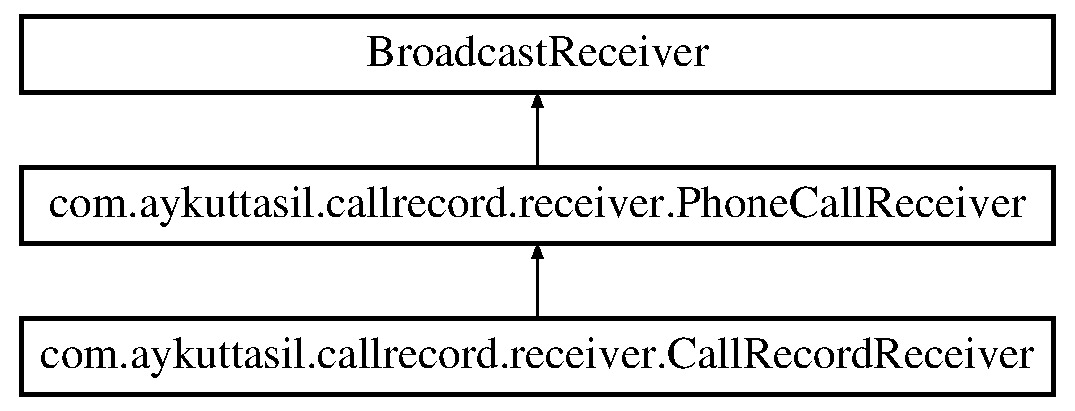
\includegraphics[height=3.000000cm]{classcom_1_1aykuttasil_1_1callrecord_1_1receiver_1_1_call_record_receiver}
\end{center}
\end{figure}
\subsection*{Public Member Functions}
\begin{DoxyCompactItemize}
\item 
\hyperlink{classcom_1_1aykuttasil_1_1callrecord_1_1receiver_1_1_call_record_receiver_a81b445370d447ac2e2594a33eac07437}{Call\+Record\+Receiver} (\hyperlink{classcom_1_1aykuttasil_1_1callrecord_1_1_call_record}{Call\+Record} call\+Record)
\end{DoxyCompactItemize}
\subsection*{Static Public Attributes}
\begin{DoxyCompactItemize}
\item 
\mbox{\Hypertarget{classcom_1_1aykuttasil_1_1callrecord_1_1receiver_1_1_call_record_receiver_aa3e89e7d92e8523a2b473a760fd52dbf}\label{classcom_1_1aykuttasil_1_1callrecord_1_1receiver_1_1_call_record_receiver_aa3e89e7d92e8523a2b473a760fd52dbf}} 
static final String {\bfseries A\+C\+T\+I\+O\+N\+\_\+\+IN} = \char`\"{}android.\+intent.\+action.\+P\+H\+O\+N\+E\+\_\+\+S\+T\+A\+TE\char`\"{}
\item 
\mbox{\Hypertarget{classcom_1_1aykuttasil_1_1callrecord_1_1receiver_1_1_call_record_receiver_a7888c821496f5072c699e7db9934e9aa}\label{classcom_1_1aykuttasil_1_1callrecord_1_1receiver_1_1_call_record_receiver_a7888c821496f5072c699e7db9934e9aa}} 
static final String {\bfseries A\+C\+T\+I\+O\+N\+\_\+\+O\+UT} = \char`\"{}android.\+intent.\+action.\+N\+E\+W\+\_\+\+O\+U\+T\+G\+O\+I\+N\+G\+\_\+\+C\+A\+LL\char`\"{}
\item 
\mbox{\Hypertarget{classcom_1_1aykuttasil_1_1callrecord_1_1receiver_1_1_call_record_receiver_ae4f527d3dd71f59890f9d376928cb902}\label{classcom_1_1aykuttasil_1_1callrecord_1_1receiver_1_1_call_record_receiver_ae4f527d3dd71f59890f9d376928cb902}} 
static final String {\bfseries E\+X\+T\+R\+A\+\_\+\+P\+H\+O\+N\+E\+\_\+\+N\+U\+M\+B\+ER} = \char`\"{}android.\+intent.\+extra.\+P\+H\+O\+N\+E\+\_\+\+N\+U\+M\+B\+ER\char`\"{}
\end{DoxyCompactItemize}
\subsection*{Protected Member Functions}
\begin{DoxyCompactItemize}
\item 
void \hyperlink{classcom_1_1aykuttasil_1_1callrecord_1_1receiver_1_1_call_record_receiver_a221eff23b7dc251021b576b9340f625c}{on\+Incoming\+Call\+Received} (Context ctx, String number, Date start)
\item 
void \hyperlink{classcom_1_1aykuttasil_1_1callrecord_1_1receiver_1_1_call_record_receiver_ae6124f62a9e2e075c5623c36fab9df0d}{on\+Incoming\+Call\+Answered} (Context ctx, String number, Date start)
\item 
void \hyperlink{classcom_1_1aykuttasil_1_1callrecord_1_1receiver_1_1_call_record_receiver_ac3e3fc614693b39c0d4117fa8ea988ad}{on\+Incoming\+Call\+Ended} (Context ctx, String number, Date start, Date end)
\item 
void \hyperlink{classcom_1_1aykuttasil_1_1callrecord_1_1receiver_1_1_call_record_receiver_a5c093fcfd710179957bc9bf9b52b242c}{on\+Outgoing\+Call\+Started} (Context ctx, String number, Date start)
\item 
void \hyperlink{classcom_1_1aykuttasil_1_1callrecord_1_1receiver_1_1_call_record_receiver_a23ac537f3d22cf22d27b76d2c8b3d2bd}{on\+Outgoing\+Call\+Ended} (Context ctx, String number, Date start, Date end)
\item 
void \hyperlink{classcom_1_1aykuttasil_1_1callrecord_1_1receiver_1_1_call_record_receiver_a602be22f458570452b057d74d5c8b0c6}{on\+Missed\+Call} (Context ctx, String number, Date start)
\end{DoxyCompactItemize}


\subsection{Detailed Description}
Регистрация звонков. 

\begin{DoxyAuthor}{Author}
Wonder\+Worcer 
\end{DoxyAuthor}
\begin{DoxyVersion}{Version}
0.\+5 
\end{DoxyVersion}
\begin{DoxyDate}{Date}
7 марта 2017 года
\end{DoxyDate}
Класс, необходим для обработки всех возможных событий при регистрации вызовов 

\subsection{Constructor \& Destructor Documentation}
\mbox{\Hypertarget{classcom_1_1aykuttasil_1_1callrecord_1_1receiver_1_1_call_record_receiver_a81b445370d447ac2e2594a33eac07437}\label{classcom_1_1aykuttasil_1_1callrecord_1_1receiver_1_1_call_record_receiver_a81b445370d447ac2e2594a33eac07437}} 
\index{com\+::aykuttasil\+::callrecord\+::receiver\+::\+Call\+Record\+Receiver@{com\+::aykuttasil\+::callrecord\+::receiver\+::\+Call\+Record\+Receiver}!Call\+Record\+Receiver@{Call\+Record\+Receiver}}
\index{Call\+Record\+Receiver@{Call\+Record\+Receiver}!com\+::aykuttasil\+::callrecord\+::receiver\+::\+Call\+Record\+Receiver@{com\+::aykuttasil\+::callrecord\+::receiver\+::\+Call\+Record\+Receiver}}
\subsubsection{\texorpdfstring{Call\+Record\+Receiver()}{CallRecordReceiver()}}
{\footnotesize\ttfamily com.\+aykuttasil.\+callrecord.\+receiver.\+Call\+Record\+Receiver.\+Call\+Record\+Receiver (\begin{DoxyParamCaption}\item[{\hyperlink{classcom_1_1aykuttasil_1_1callrecord_1_1_call_record}{Call\+Record}}]{call\+Record }\end{DoxyParamCaption})}

Конструктор 
\begin{DoxyParams}{Parameters}
{\em call\+Record} & \\
\hline
\end{DoxyParams}


\subsection{Member Function Documentation}
\mbox{\Hypertarget{classcom_1_1aykuttasil_1_1callrecord_1_1receiver_1_1_call_record_receiver_ae6124f62a9e2e075c5623c36fab9df0d}\label{classcom_1_1aykuttasil_1_1callrecord_1_1receiver_1_1_call_record_receiver_ae6124f62a9e2e075c5623c36fab9df0d}} 
\index{com\+::aykuttasil\+::callrecord\+::receiver\+::\+Call\+Record\+Receiver@{com\+::aykuttasil\+::callrecord\+::receiver\+::\+Call\+Record\+Receiver}!on\+Incoming\+Call\+Answered@{on\+Incoming\+Call\+Answered}}
\index{on\+Incoming\+Call\+Answered@{on\+Incoming\+Call\+Answered}!com\+::aykuttasil\+::callrecord\+::receiver\+::\+Call\+Record\+Receiver@{com\+::aykuttasil\+::callrecord\+::receiver\+::\+Call\+Record\+Receiver}}
\subsubsection{\texorpdfstring{on\+Incoming\+Call\+Answered()}{onIncomingCallAnswered()}}
{\footnotesize\ttfamily void com.\+aykuttasil.\+callrecord.\+receiver.\+Call\+Record\+Receiver.\+on\+Incoming\+Call\+Answered (\begin{DoxyParamCaption}\item[{Context}]{ctx,  }\item[{String}]{number,  }\item[{Date}]{start }\end{DoxyParamCaption})\hspace{0.3cm}{\ttfamily [protected]}}

Вызывается при приеме входящего вызова с последующим стартом записи разговора, если такой режим включен 
\begin{DoxyParams}{Parameters}
{\em ctx} & контект приложения \\
\hline
{\em number} & номер телефона \\
\hline
{\em start} & время принятия вызова \\
\hline
\end{DoxyParams}
\mbox{\Hypertarget{classcom_1_1aykuttasil_1_1callrecord_1_1receiver_1_1_call_record_receiver_ac3e3fc614693b39c0d4117fa8ea988ad}\label{classcom_1_1aykuttasil_1_1callrecord_1_1receiver_1_1_call_record_receiver_ac3e3fc614693b39c0d4117fa8ea988ad}} 
\index{com\+::aykuttasil\+::callrecord\+::receiver\+::\+Call\+Record\+Receiver@{com\+::aykuttasil\+::callrecord\+::receiver\+::\+Call\+Record\+Receiver}!on\+Incoming\+Call\+Ended@{on\+Incoming\+Call\+Ended}}
\index{on\+Incoming\+Call\+Ended@{on\+Incoming\+Call\+Ended}!com\+::aykuttasil\+::callrecord\+::receiver\+::\+Call\+Record\+Receiver@{com\+::aykuttasil\+::callrecord\+::receiver\+::\+Call\+Record\+Receiver}}
\subsubsection{\texorpdfstring{on\+Incoming\+Call\+Ended()}{onIncomingCallEnded()}}
{\footnotesize\ttfamily void com.\+aykuttasil.\+callrecord.\+receiver.\+Call\+Record\+Receiver.\+on\+Incoming\+Call\+Ended (\begin{DoxyParamCaption}\item[{Context}]{ctx,  }\item[{String}]{number,  }\item[{Date}]{start,  }\item[{Date}]{end }\end{DoxyParamCaption})\hspace{0.3cm}{\ttfamily [protected]}}

Вызывается после окончания входящего вызова, необходим для остановки записи. 
\begin{DoxyParams}{Parameters}
{\em ctx} & контект приложения \\
\hline
{\em number} & номер телефона \\
\hline
{\em start} & время принятия вызова \\
\hline
{\em end} & время окончания вызова \\
\hline
\end{DoxyParams}
\mbox{\Hypertarget{classcom_1_1aykuttasil_1_1callrecord_1_1receiver_1_1_call_record_receiver_a221eff23b7dc251021b576b9340f625c}\label{classcom_1_1aykuttasil_1_1callrecord_1_1receiver_1_1_call_record_receiver_a221eff23b7dc251021b576b9340f625c}} 
\index{com\+::aykuttasil\+::callrecord\+::receiver\+::\+Call\+Record\+Receiver@{com\+::aykuttasil\+::callrecord\+::receiver\+::\+Call\+Record\+Receiver}!on\+Incoming\+Call\+Received@{on\+Incoming\+Call\+Received}}
\index{on\+Incoming\+Call\+Received@{on\+Incoming\+Call\+Received}!com\+::aykuttasil\+::callrecord\+::receiver\+::\+Call\+Record\+Receiver@{com\+::aykuttasil\+::callrecord\+::receiver\+::\+Call\+Record\+Receiver}}
\subsubsection{\texorpdfstring{on\+Incoming\+Call\+Received()}{onIncomingCallReceived()}}
{\footnotesize\ttfamily void com.\+aykuttasil.\+callrecord.\+receiver.\+Call\+Record\+Receiver.\+on\+Incoming\+Call\+Received (\begin{DoxyParamCaption}\item[{Context}]{ctx,  }\item[{String}]{number,  }\item[{Date}]{start }\end{DoxyParamCaption})\hspace{0.3cm}{\ttfamily [protected]}}

Вызывается при принятии входящего вызова На данный момент не работает 
\begin{DoxyParams}{Parameters}
{\em ctx} & контект приложения \\
\hline
{\em number} & номер телефона \\
\hline
{\em start} & время принятия вызова На данный момент не работает \\
\hline
\end{DoxyParams}
\mbox{\Hypertarget{classcom_1_1aykuttasil_1_1callrecord_1_1receiver_1_1_call_record_receiver_a602be22f458570452b057d74d5c8b0c6}\label{classcom_1_1aykuttasil_1_1callrecord_1_1receiver_1_1_call_record_receiver_a602be22f458570452b057d74d5c8b0c6}} 
\index{com\+::aykuttasil\+::callrecord\+::receiver\+::\+Call\+Record\+Receiver@{com\+::aykuttasil\+::callrecord\+::receiver\+::\+Call\+Record\+Receiver}!on\+Missed\+Call@{on\+Missed\+Call}}
\index{on\+Missed\+Call@{on\+Missed\+Call}!com\+::aykuttasil\+::callrecord\+::receiver\+::\+Call\+Record\+Receiver@{com\+::aykuttasil\+::callrecord\+::receiver\+::\+Call\+Record\+Receiver}}
\subsubsection{\texorpdfstring{on\+Missed\+Call()}{onMissedCall()}}
{\footnotesize\ttfamily void com.\+aykuttasil.\+callrecord.\+receiver.\+Call\+Record\+Receiver.\+on\+Missed\+Call (\begin{DoxyParamCaption}\item[{Context}]{ctx,  }\item[{String}]{number,  }\item[{Date}]{start }\end{DoxyParamCaption})\hspace{0.3cm}{\ttfamily [protected]}}

Возникает при пропуске звонка На данный момент не работает 
\begin{DoxyParams}{Parameters}
{\em ctx} & контект приложения \\
\hline
{\em number} & номер телефона \\
\hline
{\em start} & время принятия вызова \\
\hline
\end{DoxyParams}
\mbox{\Hypertarget{classcom_1_1aykuttasil_1_1callrecord_1_1receiver_1_1_call_record_receiver_a23ac537f3d22cf22d27b76d2c8b3d2bd}\label{classcom_1_1aykuttasil_1_1callrecord_1_1receiver_1_1_call_record_receiver_a23ac537f3d22cf22d27b76d2c8b3d2bd}} 
\index{com\+::aykuttasil\+::callrecord\+::receiver\+::\+Call\+Record\+Receiver@{com\+::aykuttasil\+::callrecord\+::receiver\+::\+Call\+Record\+Receiver}!on\+Outgoing\+Call\+Ended@{on\+Outgoing\+Call\+Ended}}
\index{on\+Outgoing\+Call\+Ended@{on\+Outgoing\+Call\+Ended}!com\+::aykuttasil\+::callrecord\+::receiver\+::\+Call\+Record\+Receiver@{com\+::aykuttasil\+::callrecord\+::receiver\+::\+Call\+Record\+Receiver}}
\subsubsection{\texorpdfstring{on\+Outgoing\+Call\+Ended()}{onOutgoingCallEnded()}}
{\footnotesize\ttfamily void com.\+aykuttasil.\+callrecord.\+receiver.\+Call\+Record\+Receiver.\+on\+Outgoing\+Call\+Ended (\begin{DoxyParamCaption}\item[{Context}]{ctx,  }\item[{String}]{number,  }\item[{Date}]{start,  }\item[{Date}]{end }\end{DoxyParamCaption})\hspace{0.3cm}{\ttfamily [protected]}}

Вызывается после окончания исходящего вызова, необходим для остановки записи. 
\begin{DoxyParams}{Parameters}
{\em ctx} & контект приложения \\
\hline
{\em number} & номер телефона \\
\hline
{\em start} & время принятия вызова \\
\hline
{\em end} & время окончания вызова \\
\hline
\end{DoxyParams}
\mbox{\Hypertarget{classcom_1_1aykuttasil_1_1callrecord_1_1receiver_1_1_call_record_receiver_a5c093fcfd710179957bc9bf9b52b242c}\label{classcom_1_1aykuttasil_1_1callrecord_1_1receiver_1_1_call_record_receiver_a5c093fcfd710179957bc9bf9b52b242c}} 
\index{com\+::aykuttasil\+::callrecord\+::receiver\+::\+Call\+Record\+Receiver@{com\+::aykuttasil\+::callrecord\+::receiver\+::\+Call\+Record\+Receiver}!on\+Outgoing\+Call\+Started@{on\+Outgoing\+Call\+Started}}
\index{on\+Outgoing\+Call\+Started@{on\+Outgoing\+Call\+Started}!com\+::aykuttasil\+::callrecord\+::receiver\+::\+Call\+Record\+Receiver@{com\+::aykuttasil\+::callrecord\+::receiver\+::\+Call\+Record\+Receiver}}
\subsubsection{\texorpdfstring{on\+Outgoing\+Call\+Started()}{onOutgoingCallStarted()}}
{\footnotesize\ttfamily void com.\+aykuttasil.\+callrecord.\+receiver.\+Call\+Record\+Receiver.\+on\+Outgoing\+Call\+Started (\begin{DoxyParamCaption}\item[{Context}]{ctx,  }\item[{String}]{number,  }\item[{Date}]{start }\end{DoxyParamCaption})\hspace{0.3cm}{\ttfamily [protected]}}

Вызывается при приеме исходящего вызова с последующим стартом записи разговора, если такой режим включен 
\begin{DoxyParams}{Parameters}
{\em ctx} & контект приложения \\
\hline
{\em number} & номер телефона \\
\hline
{\em start} & время принятия вызова \\
\hline
\end{DoxyParams}


The documentation for this class was generated from the following file\+:\begin{DoxyCompactItemize}
\item 
D\+:/\+Diplomov/\+Call\+Recorder/callrecord/src/main/java/com/aykuttasil/callrecord/receiver/Call\+Record\+Receiver.\+java\end{DoxyCompactItemize}

\hypertarget{classcom_1_1aykuttasil_1_1callrecord_1_1service_1_1_call_record_service}{}\section{com.\+aykuttasil.\+callrecord.\+service.\+Call\+Record\+Service Class Reference}
\label{classcom_1_1aykuttasil_1_1callrecord_1_1service_1_1_call_record_service}\index{com.\+aykuttasil.\+callrecord.\+service.\+Call\+Record\+Service@{com.\+aykuttasil.\+callrecord.\+service.\+Call\+Record\+Service}}


Регистрация звонков.  


Inheritance diagram for com.\+aykuttasil.\+callrecord.\+service.\+Call\+Record\+Service\+:\begin{figure}[H]
\begin{center}
\leavevmode
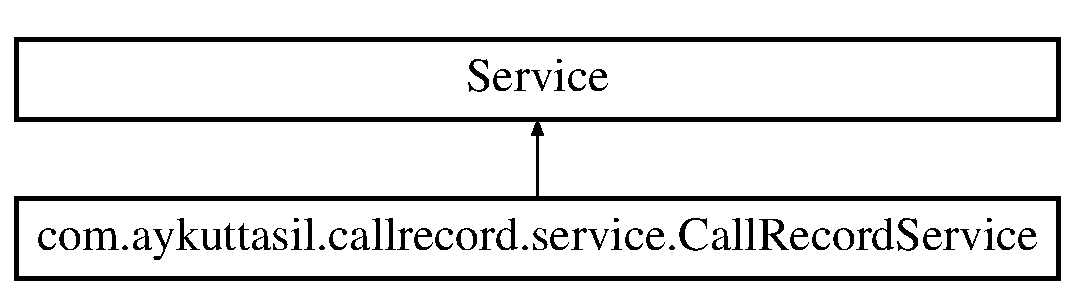
\includegraphics[height=2.000000cm]{classcom_1_1aykuttasil_1_1callrecord_1_1service_1_1_call_record_service}
\end{center}
\end{figure}
\subsection*{Public Member Functions}
\begin{DoxyCompactItemize}
\item 
I\+Binder \hyperlink{classcom_1_1aykuttasil_1_1callrecord_1_1service_1_1_call_record_service_a9093beaceb138056c7cb92d9dbe67bc4}{on\+Bind} (Intent intent)
\end{DoxyCompactItemize}


\subsection{Detailed Description}
Регистрация звонков. 

\begin{DoxyAuthor}{Author}
Wonder\+Worcer 
\end{DoxyAuthor}
\begin{DoxyVersion}{Version}
0.\+5 
\end{DoxyVersion}
\begin{DoxyDate}{Date}
7 марта 2017 года
\end{DoxyDate}
Класс, реализующий сервис записи разговора На данный момент не работает 

\subsection{Member Function Documentation}
\mbox{\Hypertarget{classcom_1_1aykuttasil_1_1callrecord_1_1service_1_1_call_record_service_a9093beaceb138056c7cb92d9dbe67bc4}\label{classcom_1_1aykuttasil_1_1callrecord_1_1service_1_1_call_record_service_a9093beaceb138056c7cb92d9dbe67bc4}} 
\index{com\+::aykuttasil\+::callrecord\+::service\+::\+Call\+Record\+Service@{com\+::aykuttasil\+::callrecord\+::service\+::\+Call\+Record\+Service}!on\+Bind@{on\+Bind}}
\index{on\+Bind@{on\+Bind}!com\+::aykuttasil\+::callrecord\+::service\+::\+Call\+Record\+Service@{com\+::aykuttasil\+::callrecord\+::service\+::\+Call\+Record\+Service}}
\subsubsection{\texorpdfstring{on\+Bind()}{onBind()}}
{\footnotesize\ttfamily I\+Binder com.\+aykuttasil.\+callrecord.\+service.\+Call\+Record\+Service.\+on\+Bind (\begin{DoxyParamCaption}\item[{Intent}]{intent }\end{DoxyParamCaption})}

Дефолтный метод, на данный момент не используется 

The documentation for this class was generated from the following file\+:\begin{DoxyCompactItemize}
\item 
D\+:/\+Diplomov/\+Call\+Recorder/callrecord/src/main/java/com/aykuttasil/callrecord/service/Call\+Record\+Service.\+java\end{DoxyCompactItemize}

\hypertarget{classcom_1_1aykuttasil_1_1callrecord_1_1receiver_1_1_phone_call_receiver}{}\section{com.\+aykuttasil.\+callrecord.\+receiver.\+Phone\+Call\+Receiver Class Reference}
\label{classcom_1_1aykuttasil_1_1callrecord_1_1receiver_1_1_phone_call_receiver}\index{com.\+aykuttasil.\+callrecord.\+receiver.\+Phone\+Call\+Receiver@{com.\+aykuttasil.\+callrecord.\+receiver.\+Phone\+Call\+Receiver}}


Регистрация звонков.  


Inheritance diagram for com.\+aykuttasil.\+callrecord.\+receiver.\+Phone\+Call\+Receiver\+:\begin{figure}[H]
\begin{center}
\leavevmode
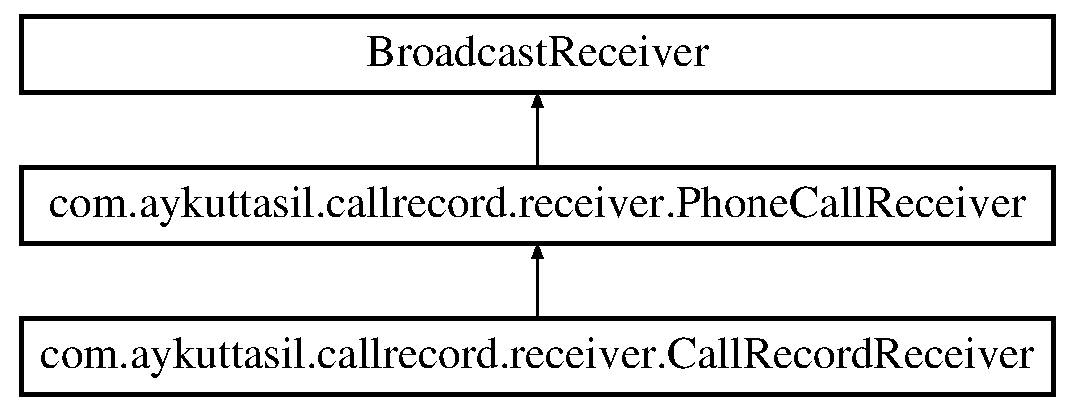
\includegraphics[height=3.000000cm]{classcom_1_1aykuttasil_1_1callrecord_1_1receiver_1_1_phone_call_receiver}
\end{center}
\end{figure}
\subsection*{Public Member Functions}
\begin{DoxyCompactItemize}
\item 
\hyperlink{classcom_1_1aykuttasil_1_1callrecord_1_1receiver_1_1_phone_call_receiver_a8573a80ead7b662c01888587a954f43c}{Phone\+Call\+Receiver} (\hyperlink{classcom_1_1aykuttasil_1_1callrecord_1_1_call_record}{Call\+Record} call\+Record)
\item 
void \hyperlink{classcom_1_1aykuttasil_1_1callrecord_1_1receiver_1_1_phone_call_receiver_afb663077b0c88ec248bd448046be73f6}{on\+Receive} (Context context, Intent intent)
\item 
void \hyperlink{classcom_1_1aykuttasil_1_1callrecord_1_1receiver_1_1_phone_call_receiver_ac2f4b48513270ed65700818b10acd5f8}{on\+Call\+State\+Changed} (Context context, int state, String number)
\end{DoxyCompactItemize}
\subsection*{Protected Member Functions}
\begin{DoxyCompactItemize}
\item 
abstract void \hyperlink{classcom_1_1aykuttasil_1_1callrecord_1_1receiver_1_1_phone_call_receiver_ae5652596a226051d4c9c17c60a33e0e9}{on\+Incoming\+Call\+Received} (Context ctx, String number, Date start)
\item 
abstract void \hyperlink{classcom_1_1aykuttasil_1_1callrecord_1_1receiver_1_1_phone_call_receiver_acbc8b7f309fb858c04d4655446382daa}{on\+Incoming\+Call\+Answered} (Context ctx, String number, Date start)
\item 
abstract void \hyperlink{classcom_1_1aykuttasil_1_1callrecord_1_1receiver_1_1_phone_call_receiver_a3a8498e884fcd5f0d9f8b1b7430b1205}{on\+Incoming\+Call\+Ended} (Context ctx, String number, Date start, Date end)
\item 
abstract void \hyperlink{classcom_1_1aykuttasil_1_1callrecord_1_1receiver_1_1_phone_call_receiver_afd2d9ccabe85671cca9b3ef0077e4d92}{on\+Outgoing\+Call\+Started} (Context ctx, String number, Date start)
\item 
abstract void \hyperlink{classcom_1_1aykuttasil_1_1callrecord_1_1receiver_1_1_phone_call_receiver_ac59381a8d49e6b7c0e99e15674c0cef3}{on\+Outgoing\+Call\+Ended} (Context ctx, String number, Date start, Date end)
\item 
abstract void \hyperlink{classcom_1_1aykuttasil_1_1callrecord_1_1receiver_1_1_phone_call_receiver_a13b659e0a07a2334da587820ae3e5996}{on\+Missed\+Call} (Context ctx, String number, Date start)
\end{DoxyCompactItemize}


\subsection{Detailed Description}
Регистрация звонков. 

\begin{DoxyAuthor}{Author}
Wonder\+Worcer 
\end{DoxyAuthor}
\begin{DoxyVersion}{Version}
0.\+5 
\end{DoxyVersion}
\begin{DoxyDate}{Date}
7 марта 2017 года
\end{DoxyDate}
Абстрактный класс, необходим для обработки всех возможных событий при регистрации вызовов Так же обрабатывает всевозможное изменение статуса вызова 

\subsection{Constructor \& Destructor Documentation}
\mbox{\Hypertarget{classcom_1_1aykuttasil_1_1callrecord_1_1receiver_1_1_phone_call_receiver_a8573a80ead7b662c01888587a954f43c}\label{classcom_1_1aykuttasil_1_1callrecord_1_1receiver_1_1_phone_call_receiver_a8573a80ead7b662c01888587a954f43c}} 
\index{com\+::aykuttasil\+::callrecord\+::receiver\+::\+Phone\+Call\+Receiver@{com\+::aykuttasil\+::callrecord\+::receiver\+::\+Phone\+Call\+Receiver}!Phone\+Call\+Receiver@{Phone\+Call\+Receiver}}
\index{Phone\+Call\+Receiver@{Phone\+Call\+Receiver}!com\+::aykuttasil\+::callrecord\+::receiver\+::\+Phone\+Call\+Receiver@{com\+::aykuttasil\+::callrecord\+::receiver\+::\+Phone\+Call\+Receiver}}
\subsubsection{\texorpdfstring{Phone\+Call\+Receiver()}{PhoneCallReceiver()}}
{\footnotesize\ttfamily com.\+aykuttasil.\+callrecord.\+receiver.\+Phone\+Call\+Receiver.\+Phone\+Call\+Receiver (\begin{DoxyParamCaption}\item[{\hyperlink{classcom_1_1aykuttasil_1_1callrecord_1_1_call_record}{Call\+Record}}]{call\+Record }\end{DoxyParamCaption})}

Конструктор 
\begin{DoxyParams}{Parameters}
{\em call\+Record} & \\
\hline
\end{DoxyParams}


\subsection{Member Function Documentation}
\mbox{\Hypertarget{classcom_1_1aykuttasil_1_1callrecord_1_1receiver_1_1_phone_call_receiver_ac2f4b48513270ed65700818b10acd5f8}\label{classcom_1_1aykuttasil_1_1callrecord_1_1receiver_1_1_phone_call_receiver_ac2f4b48513270ed65700818b10acd5f8}} 
\index{com\+::aykuttasil\+::callrecord\+::receiver\+::\+Phone\+Call\+Receiver@{com\+::aykuttasil\+::callrecord\+::receiver\+::\+Phone\+Call\+Receiver}!on\+Call\+State\+Changed@{on\+Call\+State\+Changed}}
\index{on\+Call\+State\+Changed@{on\+Call\+State\+Changed}!com\+::aykuttasil\+::callrecord\+::receiver\+::\+Phone\+Call\+Receiver@{com\+::aykuttasil\+::callrecord\+::receiver\+::\+Phone\+Call\+Receiver}}
\subsubsection{\texorpdfstring{on\+Call\+State\+Changed()}{onCallStateChanged()}}
{\footnotesize\ttfamily void com.\+aykuttasil.\+callrecord.\+receiver.\+Phone\+Call\+Receiver.\+on\+Call\+State\+Changed (\begin{DoxyParamCaption}\item[{Context}]{context,  }\item[{int}]{state,  }\item[{String}]{number }\end{DoxyParamCaption})}

Вызывается при смене статуса звонка 
\begin{DoxyParams}{Parameters}
{\em context} & текущий контекст приложения \\
\hline
{\em state} & статус звонка 0 -\/ конец звонка (C\+A\+L\+L\+\_\+\+S\+T\+A\+T\+E\+\_\+\+I\+D\+LE) 1 -\/ звонок (C\+A\+L\+L\+\_\+\+S\+T\+A\+T\+E\+\_\+\+R\+I\+N\+G\+I\+NG) 2 -\/ звонок на удержании (C\+A\+L\+L\+\_\+\+S\+T\+A\+T\+E\+\_\+\+O\+F\+F\+H\+O\+OK) Остальные варианты статуса в программе не присутствуют \\
\hline
{\em number} & номер телефона \\
\hline
\end{DoxyParams}
\mbox{\Hypertarget{classcom_1_1aykuttasil_1_1callrecord_1_1receiver_1_1_phone_call_receiver_acbc8b7f309fb858c04d4655446382daa}\label{classcom_1_1aykuttasil_1_1callrecord_1_1receiver_1_1_phone_call_receiver_acbc8b7f309fb858c04d4655446382daa}} 
\index{com\+::aykuttasil\+::callrecord\+::receiver\+::\+Phone\+Call\+Receiver@{com\+::aykuttasil\+::callrecord\+::receiver\+::\+Phone\+Call\+Receiver}!on\+Incoming\+Call\+Answered@{on\+Incoming\+Call\+Answered}}
\index{on\+Incoming\+Call\+Answered@{on\+Incoming\+Call\+Answered}!com\+::aykuttasil\+::callrecord\+::receiver\+::\+Phone\+Call\+Receiver@{com\+::aykuttasil\+::callrecord\+::receiver\+::\+Phone\+Call\+Receiver}}
\subsubsection{\texorpdfstring{on\+Incoming\+Call\+Answered()}{onIncomingCallAnswered()}}
{\footnotesize\ttfamily abstract void com.\+aykuttasil.\+callrecord.\+receiver.\+Phone\+Call\+Receiver.\+on\+Incoming\+Call\+Answered (\begin{DoxyParamCaption}\item[{Context}]{ctx,  }\item[{String}]{number,  }\item[{Date}]{start }\end{DoxyParamCaption})\hspace{0.3cm}{\ttfamily [abstract]}, {\ttfamily [protected]}}

Вызывается при приеме входящего вызова с последующим стартом записи разговора, если такой режим включен 
\begin{DoxyParams}{Parameters}
{\em ctx} & контект приложения \\
\hline
{\em number} & номер телефона \\
\hline
{\em start} & время принятия вызова \\
\hline
\end{DoxyParams}
\mbox{\Hypertarget{classcom_1_1aykuttasil_1_1callrecord_1_1receiver_1_1_phone_call_receiver_a3a8498e884fcd5f0d9f8b1b7430b1205}\label{classcom_1_1aykuttasil_1_1callrecord_1_1receiver_1_1_phone_call_receiver_a3a8498e884fcd5f0d9f8b1b7430b1205}} 
\index{com\+::aykuttasil\+::callrecord\+::receiver\+::\+Phone\+Call\+Receiver@{com\+::aykuttasil\+::callrecord\+::receiver\+::\+Phone\+Call\+Receiver}!on\+Incoming\+Call\+Ended@{on\+Incoming\+Call\+Ended}}
\index{on\+Incoming\+Call\+Ended@{on\+Incoming\+Call\+Ended}!com\+::aykuttasil\+::callrecord\+::receiver\+::\+Phone\+Call\+Receiver@{com\+::aykuttasil\+::callrecord\+::receiver\+::\+Phone\+Call\+Receiver}}
\subsubsection{\texorpdfstring{on\+Incoming\+Call\+Ended()}{onIncomingCallEnded()}}
{\footnotesize\ttfamily abstract void com.\+aykuttasil.\+callrecord.\+receiver.\+Phone\+Call\+Receiver.\+on\+Incoming\+Call\+Ended (\begin{DoxyParamCaption}\item[{Context}]{ctx,  }\item[{String}]{number,  }\item[{Date}]{start,  }\item[{Date}]{end }\end{DoxyParamCaption})\hspace{0.3cm}{\ttfamily [abstract]}, {\ttfamily [protected]}}

Вызывается после окончания входящего вызова, необходим для остановки записи. 
\begin{DoxyParams}{Parameters}
{\em ctx} & контект приложения \\
\hline
{\em number} & номер телефона \\
\hline
{\em start} & время принятия вызова \\
\hline
{\em end} & время окончания вызова \\
\hline
\end{DoxyParams}
\mbox{\Hypertarget{classcom_1_1aykuttasil_1_1callrecord_1_1receiver_1_1_phone_call_receiver_ae5652596a226051d4c9c17c60a33e0e9}\label{classcom_1_1aykuttasil_1_1callrecord_1_1receiver_1_1_phone_call_receiver_ae5652596a226051d4c9c17c60a33e0e9}} 
\index{com\+::aykuttasil\+::callrecord\+::receiver\+::\+Phone\+Call\+Receiver@{com\+::aykuttasil\+::callrecord\+::receiver\+::\+Phone\+Call\+Receiver}!on\+Incoming\+Call\+Received@{on\+Incoming\+Call\+Received}}
\index{on\+Incoming\+Call\+Received@{on\+Incoming\+Call\+Received}!com\+::aykuttasil\+::callrecord\+::receiver\+::\+Phone\+Call\+Receiver@{com\+::aykuttasil\+::callrecord\+::receiver\+::\+Phone\+Call\+Receiver}}
\subsubsection{\texorpdfstring{on\+Incoming\+Call\+Received()}{onIncomingCallReceived()}}
{\footnotesize\ttfamily abstract void com.\+aykuttasil.\+callrecord.\+receiver.\+Phone\+Call\+Receiver.\+on\+Incoming\+Call\+Received (\begin{DoxyParamCaption}\item[{Context}]{ctx,  }\item[{String}]{number,  }\item[{Date}]{start }\end{DoxyParamCaption})\hspace{0.3cm}{\ttfamily [abstract]}, {\ttfamily [protected]}}

Вызывается при принятии входящего вызова На данный момент не работает 
\begin{DoxyParams}{Parameters}
{\em ctx} & контект приложения \\
\hline
{\em number} & номер телефона \\
\hline
{\em start} & время принятия вызова На данный момент не работает \\
\hline
\end{DoxyParams}
\mbox{\Hypertarget{classcom_1_1aykuttasil_1_1callrecord_1_1receiver_1_1_phone_call_receiver_a13b659e0a07a2334da587820ae3e5996}\label{classcom_1_1aykuttasil_1_1callrecord_1_1receiver_1_1_phone_call_receiver_a13b659e0a07a2334da587820ae3e5996}} 
\index{com\+::aykuttasil\+::callrecord\+::receiver\+::\+Phone\+Call\+Receiver@{com\+::aykuttasil\+::callrecord\+::receiver\+::\+Phone\+Call\+Receiver}!on\+Missed\+Call@{on\+Missed\+Call}}
\index{on\+Missed\+Call@{on\+Missed\+Call}!com\+::aykuttasil\+::callrecord\+::receiver\+::\+Phone\+Call\+Receiver@{com\+::aykuttasil\+::callrecord\+::receiver\+::\+Phone\+Call\+Receiver}}
\subsubsection{\texorpdfstring{on\+Missed\+Call()}{onMissedCall()}}
{\footnotesize\ttfamily abstract void com.\+aykuttasil.\+callrecord.\+receiver.\+Phone\+Call\+Receiver.\+on\+Missed\+Call (\begin{DoxyParamCaption}\item[{Context}]{ctx,  }\item[{String}]{number,  }\item[{Date}]{start }\end{DoxyParamCaption})\hspace{0.3cm}{\ttfamily [abstract]}, {\ttfamily [protected]}}

Возникает при пропуске звонка На данный момент не работает 
\begin{DoxyParams}{Parameters}
{\em ctx} & контект приложения \\
\hline
{\em number} & номер телефона \\
\hline
{\em start} & время принятия вызова \\
\hline
\end{DoxyParams}
\mbox{\Hypertarget{classcom_1_1aykuttasil_1_1callrecord_1_1receiver_1_1_phone_call_receiver_ac59381a8d49e6b7c0e99e15674c0cef3}\label{classcom_1_1aykuttasil_1_1callrecord_1_1receiver_1_1_phone_call_receiver_ac59381a8d49e6b7c0e99e15674c0cef3}} 
\index{com\+::aykuttasil\+::callrecord\+::receiver\+::\+Phone\+Call\+Receiver@{com\+::aykuttasil\+::callrecord\+::receiver\+::\+Phone\+Call\+Receiver}!on\+Outgoing\+Call\+Ended@{on\+Outgoing\+Call\+Ended}}
\index{on\+Outgoing\+Call\+Ended@{on\+Outgoing\+Call\+Ended}!com\+::aykuttasil\+::callrecord\+::receiver\+::\+Phone\+Call\+Receiver@{com\+::aykuttasil\+::callrecord\+::receiver\+::\+Phone\+Call\+Receiver}}
\subsubsection{\texorpdfstring{on\+Outgoing\+Call\+Ended()}{onOutgoingCallEnded()}}
{\footnotesize\ttfamily abstract void com.\+aykuttasil.\+callrecord.\+receiver.\+Phone\+Call\+Receiver.\+on\+Outgoing\+Call\+Ended (\begin{DoxyParamCaption}\item[{Context}]{ctx,  }\item[{String}]{number,  }\item[{Date}]{start,  }\item[{Date}]{end }\end{DoxyParamCaption})\hspace{0.3cm}{\ttfamily [abstract]}, {\ttfamily [protected]}}

Вызывается после окончания исходящего вызова, необходим для остановки записи. 
\begin{DoxyParams}{Parameters}
{\em ctx} & контект приложения \\
\hline
{\em number} & номер телефона \\
\hline
{\em start} & время принятия вызова \\
\hline
{\em end} & время окончания вызова \\
\hline
\end{DoxyParams}
\mbox{\Hypertarget{classcom_1_1aykuttasil_1_1callrecord_1_1receiver_1_1_phone_call_receiver_afd2d9ccabe85671cca9b3ef0077e4d92}\label{classcom_1_1aykuttasil_1_1callrecord_1_1receiver_1_1_phone_call_receiver_afd2d9ccabe85671cca9b3ef0077e4d92}} 
\index{com\+::aykuttasil\+::callrecord\+::receiver\+::\+Phone\+Call\+Receiver@{com\+::aykuttasil\+::callrecord\+::receiver\+::\+Phone\+Call\+Receiver}!on\+Outgoing\+Call\+Started@{on\+Outgoing\+Call\+Started}}
\index{on\+Outgoing\+Call\+Started@{on\+Outgoing\+Call\+Started}!com\+::aykuttasil\+::callrecord\+::receiver\+::\+Phone\+Call\+Receiver@{com\+::aykuttasil\+::callrecord\+::receiver\+::\+Phone\+Call\+Receiver}}
\subsubsection{\texorpdfstring{on\+Outgoing\+Call\+Started()}{onOutgoingCallStarted()}}
{\footnotesize\ttfamily abstract void com.\+aykuttasil.\+callrecord.\+receiver.\+Phone\+Call\+Receiver.\+on\+Outgoing\+Call\+Started (\begin{DoxyParamCaption}\item[{Context}]{ctx,  }\item[{String}]{number,  }\item[{Date}]{start }\end{DoxyParamCaption})\hspace{0.3cm}{\ttfamily [abstract]}, {\ttfamily [protected]}}

Вызывается при приеме исходящего вызова с последующим стартом записи разговора, если такой режим включен 
\begin{DoxyParams}{Parameters}
{\em ctx} & контект приложения \\
\hline
{\em number} & номер телефона \\
\hline
{\em start} & время принятия вызова \\
\hline
\end{DoxyParams}
\mbox{\Hypertarget{classcom_1_1aykuttasil_1_1callrecord_1_1receiver_1_1_phone_call_receiver_afb663077b0c88ec248bd448046be73f6}\label{classcom_1_1aykuttasil_1_1callrecord_1_1receiver_1_1_phone_call_receiver_afb663077b0c88ec248bd448046be73f6}} 
\index{com\+::aykuttasil\+::callrecord\+::receiver\+::\+Phone\+Call\+Receiver@{com\+::aykuttasil\+::callrecord\+::receiver\+::\+Phone\+Call\+Receiver}!on\+Receive@{on\+Receive}}
\index{on\+Receive@{on\+Receive}!com\+::aykuttasil\+::callrecord\+::receiver\+::\+Phone\+Call\+Receiver@{com\+::aykuttasil\+::callrecord\+::receiver\+::\+Phone\+Call\+Receiver}}
\subsubsection{\texorpdfstring{on\+Receive()}{onReceive()}}
{\footnotesize\ttfamily void com.\+aykuttasil.\+callrecord.\+receiver.\+Phone\+Call\+Receiver.\+on\+Receive (\begin{DoxyParamCaption}\item[{Context}]{context,  }\item[{Intent}]{intent }\end{DoxyParamCaption})}

Необходимо для проверки есть ли новый исходящий вызов, если таковой имеется запишем номер, иначе запишем номер текущего вызова, его статус 
\begin{DoxyParams}{Parameters}
{\em context} & Текущий контект приложения \\
\hline
{\em intent} & описывает операцию, которую требуется запустить, а также содержит все остальные необходимые данные. \\
\hline
\end{DoxyParams}


The documentation for this class was generated from the following file\+:\begin{DoxyCompactItemize}
\item 
D\+:/\+Diplomov/\+Call\+Recorder/callrecord/src/main/java/com/aykuttasil/callrecord/receiver/Phone\+Call\+Receiver.\+java\end{DoxyCompactItemize}

\hypertarget{classcom_1_1aykuttasil_1_1callrecord_1_1helper_1_1_prefs_helper}{}\section{com.\+aykuttasil.\+callrecord.\+helper.\+Prefs\+Helper Class Reference}
\label{classcom_1_1aykuttasil_1_1callrecord_1_1helper_1_1_prefs_helper}\index{com.\+aykuttasil.\+callrecord.\+helper.\+Prefs\+Helper@{com.\+aykuttasil.\+callrecord.\+helper.\+Prefs\+Helper}}


Регистрация звонков.  


\subsection*{Public Member Functions}
\begin{DoxyCompactItemize}
\item 
\hyperlink{classcom_1_1aykuttasil_1_1callrecord_1_1helper_1_1_prefs_helper_ab49562720e21438e0e886cbcdf955d50}{Prefs\+Helper} (Context context, String pref\+\_\+name)
\item 
\hyperlink{classcom_1_1aykuttasil_1_1callrecord_1_1helper_1_1_prefs_helper_af2af1e665783a6b36b6668899e64d4c5}{Prefs\+Helper} (Context context)
\item 
Shared\+Preferences \hyperlink{classcom_1_1aykuttasil_1_1callrecord_1_1helper_1_1_prefs_helper_ad14e4ad705aa0f59f69c9365cbfab004}{get\+Preference} ()
\item 
Shared\+Preferences.\+Editor \hyperlink{classcom_1_1aykuttasil_1_1callrecord_1_1helper_1_1_prefs_helper_a909e1c90c5a4972cdca679b39bb1badb}{get\+Pref\+Editor} ()
\end{DoxyCompactItemize}
\subsection*{Static Public Member Functions}
\begin{DoxyCompactItemize}
\item 
static Shared\+Preferences \hyperlink{classcom_1_1aykuttasil_1_1callrecord_1_1helper_1_1_prefs_helper_a76641fc5715d4412e827c933192671a8}{get\+Default\+Preference} (Context context)
\item 
static void \hyperlink{classcom_1_1aykuttasil_1_1callrecord_1_1helper_1_1_prefs_helper_a3cf23eb8e76213d5155fee0367406d59}{write\+Pref\+String} (Context context, String key, String value)
\item 
static String \hyperlink{classcom_1_1aykuttasil_1_1callrecord_1_1helper_1_1_prefs_helper_ae19f5a277e32ab8af94ddf6483638055}{read\+Pref\+String} (Context context, String key)
\item 
static void \hyperlink{classcom_1_1aykuttasil_1_1callrecord_1_1helper_1_1_prefs_helper_a2fbd2a41d2ba031c9e1f0031364a970b}{write\+Pref\+Int} (Context context, String key, int value)
\item 
static int \hyperlink{classcom_1_1aykuttasil_1_1callrecord_1_1helper_1_1_prefs_helper_af5d55ee9a54f2d21b1d46b48c58653a3}{read\+Pref\+Int} (Context context, String key)
\item 
static void \hyperlink{classcom_1_1aykuttasil_1_1callrecord_1_1helper_1_1_prefs_helper_a150a57350ee1b4ba0f3d4c03cecc52b3}{write\+Pref\+Bool} (Context context, String key, boolean value)
\item 
static boolean \hyperlink{classcom_1_1aykuttasil_1_1callrecord_1_1helper_1_1_prefs_helper_a8c9acf31069d845c987e1f1dfe5b6e40}{read\+Pref\+Bool} (Context context, String key)
\item 
static void \hyperlink{classcom_1_1aykuttasil_1_1callrecord_1_1helper_1_1_prefs_helper_a96d6039f112bd5e5f945c30566019084}{clear\+Preference} (Context context)
\end{DoxyCompactItemize}


\subsection{Detailed Description}
Регистрация звонков. 

\begin{DoxyAuthor}{Author}
Wonder\+Worcer 
\end{DoxyAuthor}
\begin{DoxyVersion}{Version}
0.\+5 
\end{DoxyVersion}
\begin{DoxyDate}{Date}
7 марта 2017 года
\end{DoxyDate}
Класс, необходим для записи настроек пользователя в контекст и изменения самим приложением контекста 

\subsection{Constructor \& Destructor Documentation}
\mbox{\Hypertarget{classcom_1_1aykuttasil_1_1callrecord_1_1helper_1_1_prefs_helper_ab49562720e21438e0e886cbcdf955d50}\label{classcom_1_1aykuttasil_1_1callrecord_1_1helper_1_1_prefs_helper_ab49562720e21438e0e886cbcdf955d50}} 
\index{com\+::aykuttasil\+::callrecord\+::helper\+::\+Prefs\+Helper@{com\+::aykuttasil\+::callrecord\+::helper\+::\+Prefs\+Helper}!Prefs\+Helper@{Prefs\+Helper}}
\index{Prefs\+Helper@{Prefs\+Helper}!com\+::aykuttasil\+::callrecord\+::helper\+::\+Prefs\+Helper@{com\+::aykuttasil\+::callrecord\+::helper\+::\+Prefs\+Helper}}
\subsubsection{\texorpdfstring{Prefs\+Helper()}{PrefsHelper()}\hspace{0.1cm}{\footnotesize\ttfamily [1/2]}}
{\footnotesize\ttfamily com.\+aykuttasil.\+callrecord.\+helper.\+Prefs\+Helper.\+Prefs\+Helper (\begin{DoxyParamCaption}\item[{Context}]{context,  }\item[{String}]{pref\+\_\+name }\end{DoxyParamCaption})}


\begin{DoxyParams}{Parameters}
{\em context} & текущий контект приложения \\
\hline
{\em pref\+\_\+name} & \\
\hline
\end{DoxyParams}
\mbox{\Hypertarget{classcom_1_1aykuttasil_1_1callrecord_1_1helper_1_1_prefs_helper_af2af1e665783a6b36b6668899e64d4c5}\label{classcom_1_1aykuttasil_1_1callrecord_1_1helper_1_1_prefs_helper_af2af1e665783a6b36b6668899e64d4c5}} 
\index{com\+::aykuttasil\+::callrecord\+::helper\+::\+Prefs\+Helper@{com\+::aykuttasil\+::callrecord\+::helper\+::\+Prefs\+Helper}!Prefs\+Helper@{Prefs\+Helper}}
\index{Prefs\+Helper@{Prefs\+Helper}!com\+::aykuttasil\+::callrecord\+::helper\+::\+Prefs\+Helper@{com\+::aykuttasil\+::callrecord\+::helper\+::\+Prefs\+Helper}}
\subsubsection{\texorpdfstring{Prefs\+Helper()}{PrefsHelper()}\hspace{0.1cm}{\footnotesize\ttfamily [2/2]}}
{\footnotesize\ttfamily com.\+aykuttasil.\+callrecord.\+helper.\+Prefs\+Helper.\+Prefs\+Helper (\begin{DoxyParamCaption}\item[{Context}]{context }\end{DoxyParamCaption})}


\begin{DoxyParams}{Parameters}
{\em context} & текущий контект приложения \\
\hline
\end{DoxyParams}


\subsection{Member Function Documentation}
\mbox{\Hypertarget{classcom_1_1aykuttasil_1_1callrecord_1_1helper_1_1_prefs_helper_a96d6039f112bd5e5f945c30566019084}\label{classcom_1_1aykuttasil_1_1callrecord_1_1helper_1_1_prefs_helper_a96d6039f112bd5e5f945c30566019084}} 
\index{com\+::aykuttasil\+::callrecord\+::helper\+::\+Prefs\+Helper@{com\+::aykuttasil\+::callrecord\+::helper\+::\+Prefs\+Helper}!clear\+Preference@{clear\+Preference}}
\index{clear\+Preference@{clear\+Preference}!com\+::aykuttasil\+::callrecord\+::helper\+::\+Prefs\+Helper@{com\+::aykuttasil\+::callrecord\+::helper\+::\+Prefs\+Helper}}
\subsubsection{\texorpdfstring{clear\+Preference()}{clearPreference()}}
{\footnotesize\ttfamily static void com.\+aykuttasil.\+callrecord.\+helper.\+Prefs\+Helper.\+clear\+Preference (\begin{DoxyParamCaption}\item[{Context}]{context }\end{DoxyParamCaption})\hspace{0.3cm}{\ttfamily [static]}}

Отчищает контекст от пользовательских настроек 
\begin{DoxyParams}{Parameters}
{\em context} & текущий контект приложения \\
\hline
\end{DoxyParams}
\mbox{\Hypertarget{classcom_1_1aykuttasil_1_1callrecord_1_1helper_1_1_prefs_helper_a76641fc5715d4412e827c933192671a8}\label{classcom_1_1aykuttasil_1_1callrecord_1_1helper_1_1_prefs_helper_a76641fc5715d4412e827c933192671a8}} 
\index{com\+::aykuttasil\+::callrecord\+::helper\+::\+Prefs\+Helper@{com\+::aykuttasil\+::callrecord\+::helper\+::\+Prefs\+Helper}!get\+Default\+Preference@{get\+Default\+Preference}}
\index{get\+Default\+Preference@{get\+Default\+Preference}!com\+::aykuttasil\+::callrecord\+::helper\+::\+Prefs\+Helper@{com\+::aykuttasil\+::callrecord\+::helper\+::\+Prefs\+Helper}}
\subsubsection{\texorpdfstring{get\+Default\+Preference()}{getDefaultPreference()}}
{\footnotesize\ttfamily static Shared\+Preferences com.\+aykuttasil.\+callrecord.\+helper.\+Prefs\+Helper.\+get\+Default\+Preference (\begin{DoxyParamCaption}\item[{Context}]{context }\end{DoxyParamCaption})\hspace{0.3cm}{\ttfamily [static]}}


\begin{DoxyParams}{Parameters}
{\em context} & текущий контект приложения \\
\hline
\end{DoxyParams}
\begin{DoxyReturn}{Returns}

\end{DoxyReturn}
\mbox{\Hypertarget{classcom_1_1aykuttasil_1_1callrecord_1_1helper_1_1_prefs_helper_a909e1c90c5a4972cdca679b39bb1badb}\label{classcom_1_1aykuttasil_1_1callrecord_1_1helper_1_1_prefs_helper_a909e1c90c5a4972cdca679b39bb1badb}} 
\index{com\+::aykuttasil\+::callrecord\+::helper\+::\+Prefs\+Helper@{com\+::aykuttasil\+::callrecord\+::helper\+::\+Prefs\+Helper}!get\+Pref\+Editor@{get\+Pref\+Editor}}
\index{get\+Pref\+Editor@{get\+Pref\+Editor}!com\+::aykuttasil\+::callrecord\+::helper\+::\+Prefs\+Helper@{com\+::aykuttasil\+::callrecord\+::helper\+::\+Prefs\+Helper}}
\subsubsection{\texorpdfstring{get\+Pref\+Editor()}{getPrefEditor()}}
{\footnotesize\ttfamily Shared\+Preferences.\+Editor com.\+aykuttasil.\+callrecord.\+helper.\+Prefs\+Helper.\+get\+Pref\+Editor (\begin{DoxyParamCaption}{ }\end{DoxyParamCaption})}

Необходим для получения объекта, содержащего общие настройки контекста \begin{DoxyReturn}{Returns}
объект, сожержащий настройки контекста 
\end{DoxyReturn}
\mbox{\Hypertarget{classcom_1_1aykuttasil_1_1callrecord_1_1helper_1_1_prefs_helper_ad14e4ad705aa0f59f69c9365cbfab004}\label{classcom_1_1aykuttasil_1_1callrecord_1_1helper_1_1_prefs_helper_ad14e4ad705aa0f59f69c9365cbfab004}} 
\index{com\+::aykuttasil\+::callrecord\+::helper\+::\+Prefs\+Helper@{com\+::aykuttasil\+::callrecord\+::helper\+::\+Prefs\+Helper}!get\+Preference@{get\+Preference}}
\index{get\+Preference@{get\+Preference}!com\+::aykuttasil\+::callrecord\+::helper\+::\+Prefs\+Helper@{com\+::aykuttasil\+::callrecord\+::helper\+::\+Prefs\+Helper}}
\subsubsection{\texorpdfstring{get\+Preference()}{getPreference()}}
{\footnotesize\ttfamily Shared\+Preferences com.\+aykuttasil.\+callrecord.\+helper.\+Prefs\+Helper.\+get\+Preference (\begin{DoxyParamCaption}{ }\end{DoxyParamCaption})}

Необходим для получения настроек контекста \begin{DoxyReturn}{Returns}
объект, содержащий настройки текущего контекста приложения 
\end{DoxyReturn}
\mbox{\Hypertarget{classcom_1_1aykuttasil_1_1callrecord_1_1helper_1_1_prefs_helper_a8c9acf31069d845c987e1f1dfe5b6e40}\label{classcom_1_1aykuttasil_1_1callrecord_1_1helper_1_1_prefs_helper_a8c9acf31069d845c987e1f1dfe5b6e40}} 
\index{com\+::aykuttasil\+::callrecord\+::helper\+::\+Prefs\+Helper@{com\+::aykuttasil\+::callrecord\+::helper\+::\+Prefs\+Helper}!read\+Pref\+Bool@{read\+Pref\+Bool}}
\index{read\+Pref\+Bool@{read\+Pref\+Bool}!com\+::aykuttasil\+::callrecord\+::helper\+::\+Prefs\+Helper@{com\+::aykuttasil\+::callrecord\+::helper\+::\+Prefs\+Helper}}
\subsubsection{\texorpdfstring{read\+Pref\+Bool()}{readPrefBool()}}
{\footnotesize\ttfamily static boolean com.\+aykuttasil.\+callrecord.\+helper.\+Prefs\+Helper.\+read\+Pref\+Bool (\begin{DoxyParamCaption}\item[{Context}]{context,  }\item[{String}]{key }\end{DoxyParamCaption})\hspace{0.3cm}{\ttfamily [static]}}

Получает логическое значение переданного параметра из контекста 
\begin{DoxyParams}{Parameters}
{\em context} & текущий контект приложения \\
\hline
{\em key} & \\
\hline
\end{DoxyParams}
\begin{DoxyReturn}{Returns}

\end{DoxyReturn}
\mbox{\Hypertarget{classcom_1_1aykuttasil_1_1callrecord_1_1helper_1_1_prefs_helper_af5d55ee9a54f2d21b1d46b48c58653a3}\label{classcom_1_1aykuttasil_1_1callrecord_1_1helper_1_1_prefs_helper_af5d55ee9a54f2d21b1d46b48c58653a3}} 
\index{com\+::aykuttasil\+::callrecord\+::helper\+::\+Prefs\+Helper@{com\+::aykuttasil\+::callrecord\+::helper\+::\+Prefs\+Helper}!read\+Pref\+Int@{read\+Pref\+Int}}
\index{read\+Pref\+Int@{read\+Pref\+Int}!com\+::aykuttasil\+::callrecord\+::helper\+::\+Prefs\+Helper@{com\+::aykuttasil\+::callrecord\+::helper\+::\+Prefs\+Helper}}
\subsubsection{\texorpdfstring{read\+Pref\+Int()}{readPrefInt()}}
{\footnotesize\ttfamily static int com.\+aykuttasil.\+callrecord.\+helper.\+Prefs\+Helper.\+read\+Pref\+Int (\begin{DoxyParamCaption}\item[{Context}]{context,  }\item[{String}]{key }\end{DoxyParamCaption})\hspace{0.3cm}{\ttfamily [static]}}

Получает целочисленное значение переданного параметра из контекста 
\begin{DoxyParams}{Parameters}
{\em context} & текущий контект приложения \\
\hline
{\em key} & название параметра \\
\hline
\end{DoxyParams}
\begin{DoxyReturn}{Returns}

\end{DoxyReturn}
\mbox{\Hypertarget{classcom_1_1aykuttasil_1_1callrecord_1_1helper_1_1_prefs_helper_ae19f5a277e32ab8af94ddf6483638055}\label{classcom_1_1aykuttasil_1_1callrecord_1_1helper_1_1_prefs_helper_ae19f5a277e32ab8af94ddf6483638055}} 
\index{com\+::aykuttasil\+::callrecord\+::helper\+::\+Prefs\+Helper@{com\+::aykuttasil\+::callrecord\+::helper\+::\+Prefs\+Helper}!read\+Pref\+String@{read\+Pref\+String}}
\index{read\+Pref\+String@{read\+Pref\+String}!com\+::aykuttasil\+::callrecord\+::helper\+::\+Prefs\+Helper@{com\+::aykuttasil\+::callrecord\+::helper\+::\+Prefs\+Helper}}
\subsubsection{\texorpdfstring{read\+Pref\+String()}{readPrefString()}}
{\footnotesize\ttfamily static String com.\+aykuttasil.\+callrecord.\+helper.\+Prefs\+Helper.\+read\+Pref\+String (\begin{DoxyParamCaption}\item[{Context}]{context,  }\item[{String}]{key }\end{DoxyParamCaption})\hspace{0.3cm}{\ttfamily [static]}}

Получает значение переданного параметра из контекта 
\begin{DoxyParams}{Parameters}
{\em context} & текущий контект приложения \\
\hline
{\em key} & название параметра \\
\hline
\end{DoxyParams}
\begin{DoxyReturn}{Returns}

\end{DoxyReturn}
\mbox{\Hypertarget{classcom_1_1aykuttasil_1_1callrecord_1_1helper_1_1_prefs_helper_a150a57350ee1b4ba0f3d4c03cecc52b3}\label{classcom_1_1aykuttasil_1_1callrecord_1_1helper_1_1_prefs_helper_a150a57350ee1b4ba0f3d4c03cecc52b3}} 
\index{com\+::aykuttasil\+::callrecord\+::helper\+::\+Prefs\+Helper@{com\+::aykuttasil\+::callrecord\+::helper\+::\+Prefs\+Helper}!write\+Pref\+Bool@{write\+Pref\+Bool}}
\index{write\+Pref\+Bool@{write\+Pref\+Bool}!com\+::aykuttasil\+::callrecord\+::helper\+::\+Prefs\+Helper@{com\+::aykuttasil\+::callrecord\+::helper\+::\+Prefs\+Helper}}
\subsubsection{\texorpdfstring{write\+Pref\+Bool()}{writePrefBool()}}
{\footnotesize\ttfamily static void com.\+aykuttasil.\+callrecord.\+helper.\+Prefs\+Helper.\+write\+Pref\+Bool (\begin{DoxyParamCaption}\item[{Context}]{context,  }\item[{String}]{key,  }\item[{boolean}]{value }\end{DoxyParamCaption})\hspace{0.3cm}{\ttfamily [static]}}

Записывает логическое значение переданного параметра в контекст 
\begin{DoxyParams}{Parameters}
{\em context} & текущий контект приложения \\
\hline
{\em key} & название параметра \\
\hline
{\em value} & значение параметра \\
\hline
\end{DoxyParams}
\mbox{\Hypertarget{classcom_1_1aykuttasil_1_1callrecord_1_1helper_1_1_prefs_helper_a2fbd2a41d2ba031c9e1f0031364a970b}\label{classcom_1_1aykuttasil_1_1callrecord_1_1helper_1_1_prefs_helper_a2fbd2a41d2ba031c9e1f0031364a970b}} 
\index{com\+::aykuttasil\+::callrecord\+::helper\+::\+Prefs\+Helper@{com\+::aykuttasil\+::callrecord\+::helper\+::\+Prefs\+Helper}!write\+Pref\+Int@{write\+Pref\+Int}}
\index{write\+Pref\+Int@{write\+Pref\+Int}!com\+::aykuttasil\+::callrecord\+::helper\+::\+Prefs\+Helper@{com\+::aykuttasil\+::callrecord\+::helper\+::\+Prefs\+Helper}}
\subsubsection{\texorpdfstring{write\+Pref\+Int()}{writePrefInt()}}
{\footnotesize\ttfamily static void com.\+aykuttasil.\+callrecord.\+helper.\+Prefs\+Helper.\+write\+Pref\+Int (\begin{DoxyParamCaption}\item[{Context}]{context,  }\item[{String}]{key,  }\item[{int}]{value }\end{DoxyParamCaption})\hspace{0.3cm}{\ttfamily [static]}}

Записывает целочисленное значение переданного параметра в контекст 
\begin{DoxyParams}{Parameters}
{\em context} & текущий контект приложения \\
\hline
{\em key} & название параметра \\
\hline
{\em value} & значение параметра \\
\hline
\end{DoxyParams}
\mbox{\Hypertarget{classcom_1_1aykuttasil_1_1callrecord_1_1helper_1_1_prefs_helper_a3cf23eb8e76213d5155fee0367406d59}\label{classcom_1_1aykuttasil_1_1callrecord_1_1helper_1_1_prefs_helper_a3cf23eb8e76213d5155fee0367406d59}} 
\index{com\+::aykuttasil\+::callrecord\+::helper\+::\+Prefs\+Helper@{com\+::aykuttasil\+::callrecord\+::helper\+::\+Prefs\+Helper}!write\+Pref\+String@{write\+Pref\+String}}
\index{write\+Pref\+String@{write\+Pref\+String}!com\+::aykuttasil\+::callrecord\+::helper\+::\+Prefs\+Helper@{com\+::aykuttasil\+::callrecord\+::helper\+::\+Prefs\+Helper}}
\subsubsection{\texorpdfstring{write\+Pref\+String()}{writePrefString()}}
{\footnotesize\ttfamily static void com.\+aykuttasil.\+callrecord.\+helper.\+Prefs\+Helper.\+write\+Pref\+String (\begin{DoxyParamCaption}\item[{Context}]{context,  }\item[{String}]{key,  }\item[{String}]{value }\end{DoxyParamCaption})\hspace{0.3cm}{\ttfamily [static]}}

Записывает строковое значение переданного параметра в контект 
\begin{DoxyParams}{Parameters}
{\em context} & текущий контект приложения \\
\hline
{\em key} & название параметра \\
\hline
{\em value} & значение параметра \\
\hline
\end{DoxyParams}


The documentation for this class was generated from the following file\+:\begin{DoxyCompactItemize}
\item 
D\+:/\+Diplomov/\+Call\+Recorder/callrecord/src/main/java/com/aykuttasil/callrecord/helper/Prefs\+Helper.\+java\end{DoxyCompactItemize}

%--- End generated contents ---

% Index
\backmatter
\newpage
\phantomsection
\clearemptydoublepage
\addcontentsline{toc}{chapter}{Index}
\printindex

\end{document}
